% Options for packages loaded elsewhere
% Options for packages loaded elsewhere
\PassOptionsToPackage{unicode}{hyperref}
\PassOptionsToPackage{hyphens}{url}
%
\documentclass[
  a4paper,
]{scrbook}
\usepackage{xcolor}
\usepackage[left=2.54cm,right=2.54cm]{geometry}
\usepackage{amsmath,amssymb}
\setcounter{secnumdepth}{5}
\usepackage{iftex}
\ifPDFTeX
  \usepackage[T1]{fontenc}
  \usepackage[utf8]{inputenc}
  \usepackage{textcomp} % provide euro and other symbols
\else % if luatex or xetex
  \usepackage{unicode-math} % this also loads fontspec
  \defaultfontfeatures{Scale=MatchLowercase}
  \defaultfontfeatures[\rmfamily]{Ligatures=TeX,Scale=1}
\fi
\usepackage{lmodern}
\ifPDFTeX\else
  % xetex/luatex font selection
\fi
% Use upquote if available, for straight quotes in verbatim environments
\IfFileExists{upquote.sty}{\usepackage{upquote}}{}
\IfFileExists{microtype.sty}{% use microtype if available
  \usepackage[]{microtype}
  \UseMicrotypeSet[protrusion]{basicmath} % disable protrusion for tt fonts
}{}
\usepackage{setspace}
\makeatletter
\@ifundefined{KOMAClassName}{% if non-KOMA class
  \IfFileExists{parskip.sty}{%
    \usepackage{parskip}
  }{% else
    \setlength{\parindent}{0pt}
    \setlength{\parskip}{6pt plus 2pt minus 1pt}}
}{% if KOMA class
  \KOMAoptions{parskip=half}}
\makeatother
% Make \paragraph and \subparagraph free-standing
\makeatletter
\ifx\paragraph\undefined\else
  \let\oldparagraph\paragraph
  \renewcommand{\paragraph}{
    \@ifstar
      \xxxParagraphStar
      \xxxParagraphNoStar
  }
  \newcommand{\xxxParagraphStar}[1]{\oldparagraph*{#1}\mbox{}}
  \newcommand{\xxxParagraphNoStar}[1]{\oldparagraph{#1}\mbox{}}
\fi
\ifx\subparagraph\undefined\else
  \let\oldsubparagraph\subparagraph
  \renewcommand{\subparagraph}{
    \@ifstar
      \xxxSubParagraphStar
      \xxxSubParagraphNoStar
  }
  \newcommand{\xxxSubParagraphStar}[1]{\oldsubparagraph*{#1}\mbox{}}
  \newcommand{\xxxSubParagraphNoStar}[1]{\oldsubparagraph{#1}\mbox{}}
\fi
\makeatother

\usepackage{color}
\usepackage{fancyvrb}
\newcommand{\VerbBar}{|}
\newcommand{\VERB}{\Verb[commandchars=\\\{\}]}
\DefineVerbatimEnvironment{Highlighting}{Verbatim}{commandchars=\\\{\}}
% Add ',fontsize=\small' for more characters per line
\usepackage{framed}
\definecolor{shadecolor}{RGB}{255,255,255}
\newenvironment{Shaded}{\begin{snugshade}}{\end{snugshade}}
\newcommand{\AlertTok}[1]{\textcolor[rgb]{0.75,0.01,0.01}{\textbf{\colorbox[rgb]{0.97,0.90,0.90}{#1}}}}
\newcommand{\AnnotationTok}[1]{\textcolor[rgb]{0.79,0.38,0.79}{#1}}
\newcommand{\AttributeTok}[1]{\textcolor[rgb]{0.00,0.34,0.68}{#1}}
\newcommand{\BaseNTok}[1]{\textcolor[rgb]{0.69,0.50,0.00}{#1}}
\newcommand{\BuiltInTok}[1]{\textcolor[rgb]{0.39,0.29,0.61}{\textbf{#1}}}
\newcommand{\CharTok}[1]{\textcolor[rgb]{0.57,0.30,0.62}{#1}}
\newcommand{\CommentTok}[1]{\textcolor[rgb]{0.54,0.53,0.53}{#1}}
\newcommand{\CommentVarTok}[1]{\textcolor[rgb]{0.00,0.58,1.00}{#1}}
\newcommand{\ConstantTok}[1]{\textcolor[rgb]{0.67,0.33,0.00}{#1}}
\newcommand{\ControlFlowTok}[1]{\textcolor[rgb]{0.12,0.11,0.11}{\textbf{#1}}}
\newcommand{\DataTypeTok}[1]{\textcolor[rgb]{0.00,0.34,0.68}{#1}}
\newcommand{\DecValTok}[1]{\textcolor[rgb]{0.69,0.50,0.00}{#1}}
\newcommand{\DocumentationTok}[1]{\textcolor[rgb]{0.38,0.47,0.50}{#1}}
\newcommand{\ErrorTok}[1]{\textcolor[rgb]{0.75,0.01,0.01}{\underline{#1}}}
\newcommand{\ExtensionTok}[1]{\textcolor[rgb]{0.00,0.58,1.00}{\textbf{#1}}}
\newcommand{\FloatTok}[1]{\textcolor[rgb]{0.69,0.50,0.00}{#1}}
\newcommand{\FunctionTok}[1]{\textcolor[rgb]{0.39,0.29,0.61}{#1}}
\newcommand{\ImportTok}[1]{\textcolor[rgb]{1.00,0.33,0.00}{#1}}
\newcommand{\InformationTok}[1]{\textcolor[rgb]{0.69,0.50,0.00}{#1}}
\newcommand{\KeywordTok}[1]{\textcolor[rgb]{0.12,0.11,0.11}{\textbf{#1}}}
\newcommand{\NormalTok}[1]{\textcolor[rgb]{0.12,0.11,0.11}{#1}}
\newcommand{\OperatorTok}[1]{\textcolor[rgb]{0.12,0.11,0.11}{#1}}
\newcommand{\OtherTok}[1]{\textcolor[rgb]{0.00,0.43,0.16}{#1}}
\newcommand{\PreprocessorTok}[1]{\textcolor[rgb]{0.00,0.43,0.16}{#1}}
\newcommand{\RegionMarkerTok}[1]{\textcolor[rgb]{0.00,0.34,0.68}{\colorbox[rgb]{0.88,0.91,0.97}{#1}}}
\newcommand{\SpecialCharTok}[1]{\textcolor[rgb]{0.24,0.68,0.91}{#1}}
\newcommand{\SpecialStringTok}[1]{\textcolor[rgb]{1.00,0.33,0.00}{#1}}
\newcommand{\StringTok}[1]{\textcolor[rgb]{0.75,0.01,0.01}{#1}}
\newcommand{\VariableTok}[1]{\textcolor[rgb]{0.00,0.34,0.68}{#1}}
\newcommand{\VerbatimStringTok}[1]{\textcolor[rgb]{0.75,0.01,0.01}{#1}}
\newcommand{\WarningTok}[1]{\textcolor[rgb]{0.75,0.01,0.01}{#1}}

\usepackage{longtable,booktabs,array}
\usepackage{calc} % for calculating minipage widths
% Correct order of tables after \paragraph or \subparagraph
\usepackage{etoolbox}
\makeatletter
\patchcmd\longtable{\par}{\if@noskipsec\mbox{}\fi\par}{}{}
\makeatother
% Allow footnotes in longtable head/foot
\IfFileExists{footnotehyper.sty}{\usepackage{footnotehyper}}{\usepackage{footnote}}
\makesavenoteenv{longtable}
\usepackage{graphicx}
\makeatletter
\newsavebox\pandoc@box
\newcommand*\pandocbounded[1]{% scales image to fit in text height/width
  \sbox\pandoc@box{#1}%
  \Gscale@div\@tempa{\textheight}{\dimexpr\ht\pandoc@box+\dp\pandoc@box\relax}%
  \Gscale@div\@tempb{\linewidth}{\wd\pandoc@box}%
  \ifdim\@tempb\p@<\@tempa\p@\let\@tempa\@tempb\fi% select the smaller of both
  \ifdim\@tempa\p@<\p@\scalebox{\@tempa}{\usebox\pandoc@box}%
  \else\usebox{\pandoc@box}%
  \fi%
}
% Set default figure placement to htbp
\def\fps@figure{htbp}
\makeatother


% definitions for citeproc citations
\NewDocumentCommand\citeproctext{}{}
\NewDocumentCommand\citeproc{mm}{%
  \begingroup\def\citeproctext{#2}\cite{#1}\endgroup}
\makeatletter
 % allow citations to break across lines
 \let\@cite@ofmt\@firstofone
 % avoid brackets around text for \cite:
 \def\@biblabel#1{}
 \def\@cite#1#2{{#1\if@tempswa , #2\fi}}
\makeatother
\newlength{\cslhangindent}
\setlength{\cslhangindent}{1.5em}
\newlength{\csllabelwidth}
\setlength{\csllabelwidth}{3em}
\newenvironment{CSLReferences}[2] % #1 hanging-indent, #2 entry-spacing
 {\begin{list}{}{%
  \setlength{\itemindent}{0pt}
  \setlength{\leftmargin}{0pt}
  \setlength{\parsep}{0pt}
  % turn on hanging indent if param 1 is 1
  \ifodd #1
   \setlength{\leftmargin}{\cslhangindent}
   \setlength{\itemindent}{-1\cslhangindent}
  \fi
  % set entry spacing
  \setlength{\itemsep}{#2\baselineskip}}}
 {\end{list}}
\usepackage{calc}
\newcommand{\CSLBlock}[1]{\hfill\break\parbox[t]{\linewidth}{\strut\ignorespaces#1\strut}}
\newcommand{\CSLLeftMargin}[1]{\parbox[t]{\csllabelwidth}{\strut#1\strut}}
\newcommand{\CSLRightInline}[1]{\parbox[t]{\linewidth - \csllabelwidth}{\strut#1\strut}}
\newcommand{\CSLIndent}[1]{\hspace{\cslhangindent}#1}



\setlength{\emergencystretch}{3em} % prevent overfull lines

\providecommand{\tightlist}{%
  \setlength{\itemsep}{0pt}\setlength{\parskip}{0pt}}



 



% add a dummy abstract environment that is defined in quarto manuscript 
% but not in the quarto book that we run first to give it a slot in the 
% side bar
\ifcsmacro{abstract}{}{
  \let\endmyenvironment\undefined%
  \newenvironment{abstract}{\chapter*{Abstract}}{}
}

% restart chapter numbers in each part
\makeatletter
\@addtoreset{chapter}{part}
\makeatother
\makeatletter
\@ifpackageloaded{caption}{}{\usepackage{caption}}
\AtBeginDocument{%
\ifdefined\contentsname
  \renewcommand*\contentsname{Table of contents}
\else
  \newcommand\contentsname{Table of contents}
\fi
\ifdefined\listfigurename
  \renewcommand*\listfigurename{List of Figures}
\else
  \newcommand\listfigurename{List of Figures}
\fi
\ifdefined\listtablename
  \renewcommand*\listtablename{List of Tables}
\else
  \newcommand\listtablename{List of Tables}
\fi
\ifdefined\figurename
  \renewcommand*\figurename{Figure}
\else
  \newcommand\figurename{Figure}
\fi
\ifdefined\tablename
  \renewcommand*\tablename{Table}
\else
  \newcommand\tablename{Table}
\fi
}
\@ifpackageloaded{float}{}{\usepackage{float}}
\floatstyle{ruled}
\@ifundefined{c@chapter}{\newfloat{codelisting}{h}{lop}}{\newfloat{codelisting}{h}{lop}[chapter]}
\floatname{codelisting}{Listing}
\newcommand*\listoflistings{\listof{codelisting}{List of Listings}}
\makeatother
\makeatletter
\makeatother
\makeatletter
\@ifpackageloaded{caption}{}{\usepackage{caption}}
\@ifpackageloaded{subcaption}{}{\usepackage{subcaption}}
\makeatother
\usepackage{bookmark}
\IfFileExists{xurl.sty}{\usepackage{xurl}}{} % add URL line breaks if available
\urlstyle{same}
\hypersetup{
  pdftitle={Notes to paperes},
  pdfkeywords={Vestibulum, Nunc ac dignissim, Proin feugiat},
  hidelinks,
  pdfcreator={LaTeX via pandoc}}


\title{Notes to paperes}
\usepackage{etoolbox}
\makeatletter
\providecommand{\subtitle}[1]{% add subtitle to \maketitle
  \apptocmd{\@title}{\par {\large #1 \par}}{}{}
}
\makeatother
\subtitle{Some subtitle for my thesis}
\author{Johan Ulstrup}
\date{August 14, 2025}
\begin{document}
\frontmatter
\maketitle

\renewcommand*\contentsname{Table of contents}
{
\setcounter{tocdepth}{1}
\tableofcontents
}

\setstretch{1}
\mainmatter
\chapter{index}\label{index}

\chapter{DNA language models are powerful predictors of genome-wide
variant
effects}\label{dna-language-models-are-powerful-predictors-of-genome-wide-variant-effects}

The idea for this project was to evaluate the Genome-Pretrained Network
(GPN) introduced in (Benegas, Batra, and Song 2024) and determine
whether it could achieve greater accuracy than traditional methods in
predicting genome-wide variant effects.

The model is designed as a convolutional neural network (CNN) and takes
input sequences with a window size of 512. During training, 15\% of the
positions within each window are masked to enable the model to learn
meaningful representations.

The architecture consists of 25 layers, each structured as follows: a
dilated convolution layer, followed by an add-and-norm layer with a skip
connection from before the dilated convolution. This is followed by a
feedforward layer, another add-and-norm layer, and additional skip
connections.

A feedforward layer is a fundamental component of neural networks, where
inputs pass through one or more fully connected layers with activation
functions, transforming data without looping back. This structure helps
the model learn complex representations by applying weighted
transformations and non-linearities.

A dilated convolution expands the receptive field of a convolutional
layer without increasing the number of parameters or reducing
resolution. By spacing kernel elements apart, it captures long-range
dependencies in sequences, making it particularly useful in genomic data
analysis. When combined, dilated convolutions and feedforward layers
enhance a model's ability to recognize patterns across different scales
efficiently.

After passing through the 25 layers, the model produces a contextual
embedding with a dimension of 512 (D=512), followed by classification
layers. The final layer outputs the probabilities of the four
nucleotides at each masked position.

The GPN variant effect prediction score is calculated as the
log-likelihood ratio between the alternate (ALT) and reference (REF)
alleles. Here, L represents the window length in base pairs, and D
denotes the embedding dimension.

\chapter{evolution on X}\label{evolution-on-x}

The production of gametes in sexually reproducing organisms is a
complex, tightly regulated process involving numerous cellular and
molecular mechanisms. In males, spermatogenesis---the process by which
sperm are formed---progresses through four main stages of
differentiation: from germ cells to spermatogonia, then to pachytene
spermatocytes, round spermatids, and finally to mature spermatozoa
\cite{Wang2019}(Wang et al.~2019). This process is fundamental to male
fertility. Meiosis, a specialized form of cell division, ensures the
proper pairing, recombination, and segregation of homologous
chromosomes, thereby maintaining genetic integrity and promoting
variation. A deep understanding of these molecular events is essential
for comprehending inheritance, speciation, population genetics, and the
biological causes of infertility.

Sex chromosomes differ from autosomes in several key ways due to their
distinct patterns of inheritance and copy number. The Y chromosome is
found only in males and exists as a single copy. In contrast, the X
chromosome follows a more complex inheritance pattern: females carry two
copies, while males carry only one. Consequently, the X chromosome
resides two-thirds of the time in females and one-third in males, a
distribution that influences how selection acts upon it. In males, the
hemizygous nature of the X chromosome means that any mutations or
deleterious alleles are fully exposed, without a second copy to mask
their effects.

This feature is central to Haldane's rule \cite{Haldane1922} (Haldane
1922), which posits that in hybrids between two species, the
heterogametic sex (e.g., XY in mammals or ZW in birds) is more likely to
be inviable or sterile. While widely observed, the precise causes of
this pattern remain a subject of ongoing debate. Several hypotheses have
been proposed to explain it. One suggests that incompatibilities
involving the Y chromosome can arise if it fails to remain compatible
with the X chromosome or autosomes. Another centers on dosage
compensation, proposing that hybridization may disrupt the regulatory
mechanisms that balance gene expression between sex chromosomes. The
dominance hypothesis argues that recessive deleterious alleles may be
unmasked in the heterogametic sex, leading to sterility. Additional
ideas include the faster evolution of male-biased reproductive genes,
which can result in functional mismatches, and the accelerated
divergence of X-linked loci compared to autosomes, known as faster-X
evolution. Lastly, meiotic drive---genetic conflicts between selfish
elements on sex chromosomes---has also been implicated in hybrid
sterility.

These hypotheses underscore the complex interplay between sex
chromosomes, selection, and hybridization \cite{Cowell2023} (Cowell
2023). Although Haldane's rule is consistently observed across diverse
taxa---and even across kingdoms---the underlying mechanisms are not
universally agreed upon. In many cases, multiple processes may act
together \cite{Lindholm2016} (Lindholm et al.~2016).

The X chromosome, in particular, appears to be subject to strong and
unique selective pressures, especially in primates. This topic is
explored in greater depth in the following sections.

\chapter{Chromatin structure}\label{chromatin-structure}

Regions under strong selection across primate species---including humans
and baboons---are consistently found on the X chromosome, spanning
megabase-scale genomic areas. As previously noted, factors such as
chromosomal architecture and structural rearrangements may play crucial
roles in enabling, regulating, or insulating these regions from
selective pressures.

Understanding genome organization and variation is therefore essential
for uncovering the mechanisms behind selection. Chromatin has long been
recognized as central to gene regulation and cellular function
(Lieberman-Aiden et al.~2009), in part because the 3D structure of
chromosomes brings distant genomic elements into close contact.
Disruption of this spatial organization can lead to developmental
abnormalities \cite{Dixon2015} (Dixon et al.~2015). Chromatin is
organized hierarchically, with multiple levels of structure nested
within one another (see Figure 2). At the broadest level, chromatin
compartments can span several megabases \cite{LiebermanAiden2009}
(Lieberman-Aiden et al.~2009), while at finer scales, even 500 base
pairs can contribute to subgenic structural organization. Structures
such as topologically associating domains (TADs) and chromatin loops,
which operate at sub-megabase scales, further help partition regulatory
elements and maintain proper genomic function
\cite{Ramirez2018}\cite{Zuo2021}(Ramírez et al.~2018; Zuo et al.~2021).

kigger på cromatin overgange er der noget der er anderledens i de
områder konseveret er der noge specifikke motiver diversiteten

Chromatin, the complex of DNA wrapped around histone proteins and
associated with various regulatory factors, plays a central role in the
spatial and temporal control of gene expression, as well as in
maintaining the structural integrity and stability of the genome. Far
from being a static scaffold, chromatin is a highly dynamic entity,
subject to extensive remodeling in response to cellular signals,
developmental cues, and environmental stimuli. Its organization within
the nucleus is hierarchical, ranging from nucleosomes to higher-order
domains, and this architecture can differ substantially across cell
types, developmental stages, and even between closely related species.
One of the key features of chromatin organization is its division into
functionally distinct states---broadly classified as euchromatin, which
is generally open and transcriptionally active, and heterochromatin,
which is compacted and repressive. Transitions between these states,
whether developmentally programmed or evolutionarily emergent, are often
tightly coupled to shifts in gene regulatory activity and cellular
identity.

In this study, we focus on characterizing these chromatin state
transitions, with a particular interest in understanding how they are
distributed across the genome and whether they exhibit predictable
patterns linked to specific sequence features or regulatory elements. We
ask whether certain genomic regions are more prone to undergoing
structural reorganization and whether such regions harbor conserved
sequence motifs, epigenetic signatures, or binding sites for key
regulatory proteins. Furthermore, we investigate whether particular
chromatin configurations are disproportionately associated with genes
involved in critical biological processes or with regions of the genome
that show signatures of evolutionary constraint or adaptation.

By examining the diversity of chromatin states and transitions across
individuals and lineages, we also aim to uncover broader principles
governing chromatin architecture and its functional consequences. These
insights may inform our understanding of how chromatin organization
evolves, how it contributes to phenotypic diversity, and how its
dysregulation may underlie disease states. Ultimately, this work
contributes to a growing body of knowledge on the interplay between
genome structure, function, and evolution.

\chapter{A/B configurations}\label{ab-configurations}

One widely studied aspect of chromatin architecture is its partitioning
into A and B compartments, as revealed by Hi-C and other genome
conformation capture techniques. These compartments represent
large-scale topological domains of the genome that differ markedly in
their regulatory environment and functional output. A compartments are
typically associated with euchromatic regions---open, accessible
chromatin that is rich in actively transcribed genes, regulatory
elements like enhancers and promoters, and active histone marks such as
H3K4me3 and H3K27ac. In contrast, B compartments correspond to
heterochromatic, transcriptionally repressive regions characterized by
reduced accessibility, fewer active genes, and enrichment of repressive
epigenetic marks like H3K9me3 and DNA methylation.

This spatial segregation of the genome into A and B compartments plays a
critical role in regulating which genes are expressed in a given cell or
context. Genes located in A compartments are more likely to be in close
physical proximity to other regulatory elements, transcriptional
machinery, and nuclear compartments that promote gene activation, such
as nuclear speckles. Conversely, genes embedded in B compartments are
more isolated from such transcriptional hubs and may be sequestered near
the nuclear lamina, where gene silencing is reinforced.

Importantly, the assignment of a genomic region to either an A or B
compartment is not fixed; it can shift in response to developmental
signals, environmental stress, or disease states. Such compartment
switching is a powerful mechanism of gene regulation. For example, when
a gene or regulatory locus moves from a B to an A compartment, it may
become transcriptionally activated due to its new, more permissive
chromatin environment. Likewise, genes that transition into B
compartments often show downregulation or complete silencing. These
dynamic shifts allow the cell to orchestrate complex gene expression
programs with spatial precision, integrating structural and regulatory
layers of genome function.

Moreover, comparative studies across species and populations suggest
that A/B compartmentalization is both conserved and evolutionarily
flexible. Certain compartments---particularly those associated with
developmental and housekeeping genes---are stably maintained across
evolutionary time, reflecting strong selective pressure to preserve core
regulatory networks. Other regions, especially those involved in
species-specific traits or environmental responses, exhibit greater
compartmental plasticity. By studying the distribution and dynamics of
A/B compartments, especially in non-model organisms and hybrid genomes,
we can gain novel insights into how chromatin structure evolves and how
it contributes to phenotypic diversity and adaptation.

\chapter{GPN}\label{gpn}

Recent advances in artificial intelligence have brought powerful tools
to genomics, particularly through the development of Genomic Pre-trained
Networks (GPNs)---deep learning models trained on large-scale genomic
sequence data using architectures inspired by natural language
processing. GPNs apply self-supervised learning approaches, analogous to
models like BERT or GPT, to the DNA sequence, learning to predict masked
or missing bases in context. Through this training, GPNs develop an
internal representation of the ``language of the genome,'' capturing
patterns of sequence composition, motif syntax, and long-range
dependencies that underlie regulatory function.

A key advantage of GPNs lies in their use of transformer architectures,
which differ significantly from traditional models like convolutional
neural networks (CNNs). While CNNs are adept at recognizing short,
fixed-length patterns---such as transcription factor binding
motifs---they struggle with learning dependencies over long genomic
distances, such as enhancer-promoter interactions or 3D chromatin
looping. Transformers, in contrast, leverage self-attention mechanisms,
which allow the model to compare and weigh relationships between all
nucleotide positions in a sequence, regardless of distance. This makes
them exceptionally well-suited for modeling the complex, multi-scale
structure of regulatory DNA.

The utility of GPNs in functional genomics has been demonstrated in
tasks such as predicting the effects of noncoding variants, chromatin
accessibility, and transcription factor binding. For instance, the model
introduced by Benegas and Batra (``DNA language models are powerful
predictors of genome-wide variant effects'') showed that
transformer-based GPNs outperform prior models in predicting variant
impact across a variety of cell types and epigenomic contexts, even
without explicit annotations. These models can generate base-resolution
functional predictions across the genome, enabling insight into the
likely regulatory role of any given sequence segment.

In the context of chromatin structure, GPNs hold particular promise for
identifying sequence features that influence or correlate with A/B
compartment identity. By learning patterns that distinguish sequences in
open (A) versus closed (B) chromatin, GPNs can be used to predict how
shifts in compartmentalization may arise from sequence variation.
Furthermore, these predictions can be extended across species or
populations to assess functional conservation---that is, whether a
sequence maintains regulatory potential or compartment association
despite genetic divergence.

In this study, we leverage GPN-derived embeddings and predictions to
investigate the sequence determinants of chromatin organization. We aim
to identify genomic regions where the GPN model predicts strong,
conserved regulatory activity, and determine whether these regions also
show structural stability in chromatin compartments across individuals
or hybrid genomes. This approach allows us to assess whether chromatin
transitions are driven primarily by changes in DNA sequence, or whether
other regulatory layers (e.g., epigenetic modifications, chromatin
remodelers) are required to explain shifts between A and B compartments.

Ultimately, integrating GPN predictions with chromatin conformation data
(e.g., from Hi-C) provides a powerful framework for exploring genome
function at multiple scales---from base-level regulatory logic to
large-scale nuclear organization. These models not only enhance our
ability to interpret genomic variation and conservation but also open
new avenues for studying the evolution of regulatory architecture in
systems such as primates, where hybridization and population structure
offer unique opportunities to dissect genome regulation in action.

\chapter{cnn vs transformer}\label{cnn-vs-transformer}

Convolutional Neural Networks (CNNs) have been the foundational
architecture in computer vision for over a decade. Introduced by LeCun
et al.~(1998) and popularized with the success of AlexNet (Krizhevsky et
al., 2012), CNNs exploit spatial hierarchies in image data through local
receptive fields and shared weights. Architectures such as VGGNet
(Simonyan \& Zisserman, 2015), ResNet (He et al., 2016), and
EfficientNet (Tan \& Le, 2019) have progressively improved the depth,
scalability, and performance of CNNs, enabling state-of-the-art results
in tasks such as image classification, object detection, and semantic
segmentation.

A simple Convolutional Neural Network (CNN) architecture typically
consists of several key types of layers. The first are convolutional
layers, which apply learnable filters (also known as kernels) to local
regions of the input data. These filters are designed to capture spatial
features such as edges, textures, and, as the network deepens, more
complex patterns. Following the convolutional operations, activation
functions are applied---most commonly the Rectified Linear Unit
(ReLU)---to introduce non-linearity into the model, enabling it to learn
more complex representations.

Pooling layers are another essential component of CNNs. These layers
downsample the feature maps, typically using max pooling or average
pooling, which reduces the spatial dimensions of the data while
retaining the most salient features. This not only lowers computational
requirements but also helps mitigate overfitting by providing a form of
translation invariance. Toward the end of the architecture, fully
connected layers are often used to perform high-level reasoning. These
layers integrate the features extracted by earlier layers and are
typically responsible for producing the final classification or
regression outputs.

One of the main strengths of CNNs lies in their use of local receptive
fields and weight sharing, which makes them highly effective at learning
spatial hierarchies and translation-invariant features. Even relatively
shallow CNNs can perform well on image-related tasks, particularly when
training data is limited.

CNNs offer several advantages. They are parameter-efficient due to
filter sharing, which significantly reduces the number of learnable
weights compared to fully connected networks. Their strong inductive
bias---emphasizing locality and translation invariance---makes them
particularly well-suited to visual data. Additionally, CNNs benefit from
computational efficiency, as they are compatible with highly optimized
GPU-based implementations, and they often require less data than more
recent architectures to achieve good performance.

However, CNNs also come with limitations. They tend to focus on local
features, which makes capturing long-range dependencies challenging
without additional architectural mechanisms. Their receptive field is
fixed and limited, so incorporating larger contextual information often
requires making the network deeper or using special techniques like
dilated convolutions or skip connections. Furthermore, CNN performance
can be sensitive to architectural choices such as filter sizes, layer
depth, and stride configurations, which often require manual tuning.

These challenges have inspired researchers to explore alternative
architectures, most notably Transformer models. Unlike CNNs,
Transformers are designed to model global relationships more naturally,
though often at the expense of requiring more data and computational
resources.

\chapter{Materials and Methods}\label{materials-and-methods}

Data Sources: Baboon genome datasets, known hybridization cases,
population size data.

Model and Tools: GPN model architecture and usage.

Preprocessing: Alignment, feature extraction, and data cleaning.

Entropy Calculation: Methodology for genome-wide entropy measurement.

\chapter{GPN arcitecture}\label{gpn-arcitecture}

The idea for this project was to evaluate the Genome-Pretrained Network
(GPN) introduced in \cite{Kantorovitz2024} and determine whether it
could achieve greater accuracy than traditional methods in predicting
genome-wide variant effects.

The model is designed as a convolutional neural network (CNN) and takes
input sequences with a window size of 512. During training, 15\% of the
positions within each window are masked to enable the model to learn
meaningful representations.

The architecture consists of 25 layers, each structured as follows: a
dilated convolution layer, followed by an add-and-norm layer with a skip
connection from before the dilated convolution. This is followed by a
feedforward layer, another add-and-norm layer, and additional skip
connections.

A feedforward layer is a fundamental component of neural networks, where
inputs pass through one or more fully connected layers with activation
functions, transforming data without looping back. This structure helps
the model learn complex representations by applying weighted
transformations and non-linearities.

A dilated convolution expands the receptive field of a convolutional
layer without increasing the number of parameters or reducing
resolution. By spacing kernel elements apart, it captures long-range
dependencies in sequences, making it particularly useful in genomic data
analysis. When combined, dilated convolutions and feedforward layers
enhance a model's ability to recognize patterns across different scales
efficiently.

After passing through the 25 layers, the model produces a contextual
embedding with a dimension of 512 (D=512), followed by classification
layers. The final layer outputs the probabilities of the four
nucleotides at each masked position.

The GPN variant effect prediction score is calculated as the
log-likelihood ratio between the alternate (ALT) and reference (REF)
alleles. Here, L represents the window length in base pairs, and D
denotes the embedding dimension.

\chapter{Data Preparation and Pretraining
Workflow}\label{data-preparation-and-pretraining-workflow}

To evaluate the Genome-Pretrained Network (GPN), the initial step
involved reproducing the pretraining workflow provided in the original
publication. This workflow outlines the procedure for generating a
dataset compatible with the model, specifically for masked language
modeling over genomic sequences.

Initial attempts to apply the workflow to a baboon genome dataset
encountered technical difficulties. These issues were not intrinsic to
the baboon data itself but stemmed from the implementation of the
workflow. To ensure compatibility with the model and maintain
consistency with the original study, the Anatoptis genome---used as the
reference in the published work---was selected as a pilot dataset.

After resolving the implementation issues, a dataset suitable for GPN
pretraining was successfully generated. The resulting data consisted of
masked genomic sequences, formatted according to the model's input
requirements.

\chapter{Model Execution Workflow and Hardware
Constraints}\label{model-execution-workflow-and-hardware-constraints}

Following the successful generation of a pretraining-compatible dataset,
the next step involved attempting to run the Genome-Pretrained Network
(GPN) using the available inference and training workflows. The
documentation provided on the model's GitHub repository lacked detailed
guidance, making it challenging to understand the complete execution
process and the rationale behind certain steps.

To proceed, an alternative workflow was identified---one specifically
designed for use with the Anatoptis genome. This workflow was adopted as
a reference implementation for executing the GPN model.

However, significant hardware limitations emerged during this phase. The
original study reported using four NVIDIA A100 GPUs, each equipped with
80 GB of RAM. In contrast, the available system utilized NVIDIA L43R
GPUs with 45 GB of RAM, resulting in substantial differences in
computational capacity.

As a result, attempts to execute the GPN model encountered frequent
out-of-memory (OOM) errors, particularly during forward passes through
the deeper layers of the network. These memory constraints posed a major
obstacle and significantly hindered reproducibility under the available
hardware setup.

Initial efforts to train or fine-tune the Genome-Pretrained Network
(GPN) focused on applying the workflow to a baboon genome using a
multi-GPU setup. The goal was to replicate the original training
environment, which employed four NVIDIA A100 GPUs (80 GB RAM each).
However, the available infrastructure utilized NVIDIA L43R GPUs, each
with 45 GB of RAM, which introduced several compatibility and
performance challenges.

Early testing began with the Anatoptis genome. Attempts to process the
entire genome using the Snakemake workflow were unsuccessful due to GPU
detection issues. These issues stemmed from the cluster configuration,
which prevented the Snakemake environment from correctly interfacing
with the available GPU hardware.

After resolving these initial configuration issues, the workflow was
executed with GPU support. While this improved performance, the model
began encountering memory errors after a few hours of training, even
when utilizing two to four GPUs in parallel. In an effort to overcome
these constraints, the number of GPUs was incrementally increased---from
four to six, and finally to eight---providing an aggregate of 360 GB of
GPU RAM.

Despite these efforts, the model continued to encounter out-of-memory
(OOM) errors during execution. Even with eight GPUs, the memory demands
of the GPN model remained prohibitive under the given cluster
configuration. These persistent failures highlighted a significant
limitation: the model's architecture and resource demands exceeded the
practical limits of the available hardware.

Ultimately, these constraints prevented successful execution of the GPN
model on the tested system.

Given the persistent memory limitations encountered during full-genome
processing, an alternative strategy was implemented. Rather than
inputting the entire Anatoptis genome, the data was partitioned at the
chromosome level. This allowed individual chromosomes to be processed
independently, while still allocating the full available GPU resources
(eight NVIDIA GPUs with a combined 360 GB of RAM) to each run.

This approach proved successful. When processing a single chromosome at
a time, the GPN model was able to execute without encountering
memory-related failures. As a result, contextual embeddings were
successfully generated for individual chromosomes of the Anatoptis
genome.

However, due to time constraints near the conclusion of the project
timeline, the extracted embeddings were not subjected to further
downstream analysis. Although they were successfully retrieved and
stored, no additional modeling, interpretation, or evaluation steps were
completed within the project scope.

\chapter{using HIC to extract transtion
areas}\label{using-hic-to-extract-transtion-areas}

\section{distance between the edges}\label{distance-between-the-edges}

To evaluate the availability of data across genomic distances and
mitigate potential bias in downstream analyses, we calculated reverse
cumulative counts of compartment edge half-distances. First, edges were
identified at compartment transitions between A and B (in either
direction). For each consecutive pair of such edges, we measured the
genomic distance between their start positions and divided it by two,
yielding the half-distance between edges.

We then binned these half-distances and computed the reverse cumulative
count for each bin, which represents the number of edges with
half-distances greater than or equal to that bin. This approach
effectively measures the number of edges capable of contributing data at
a given spatial scale. Using this metric allows us to normalize other
measurements by the available data density, reducing the risk that
apparent trends are driven by varying numbers of contributing edges at
different distances rather than true biological effects. Counts were
calculated up to 2 Mb to encompass the maximum observed separation.

\begin{figure}

\centering{

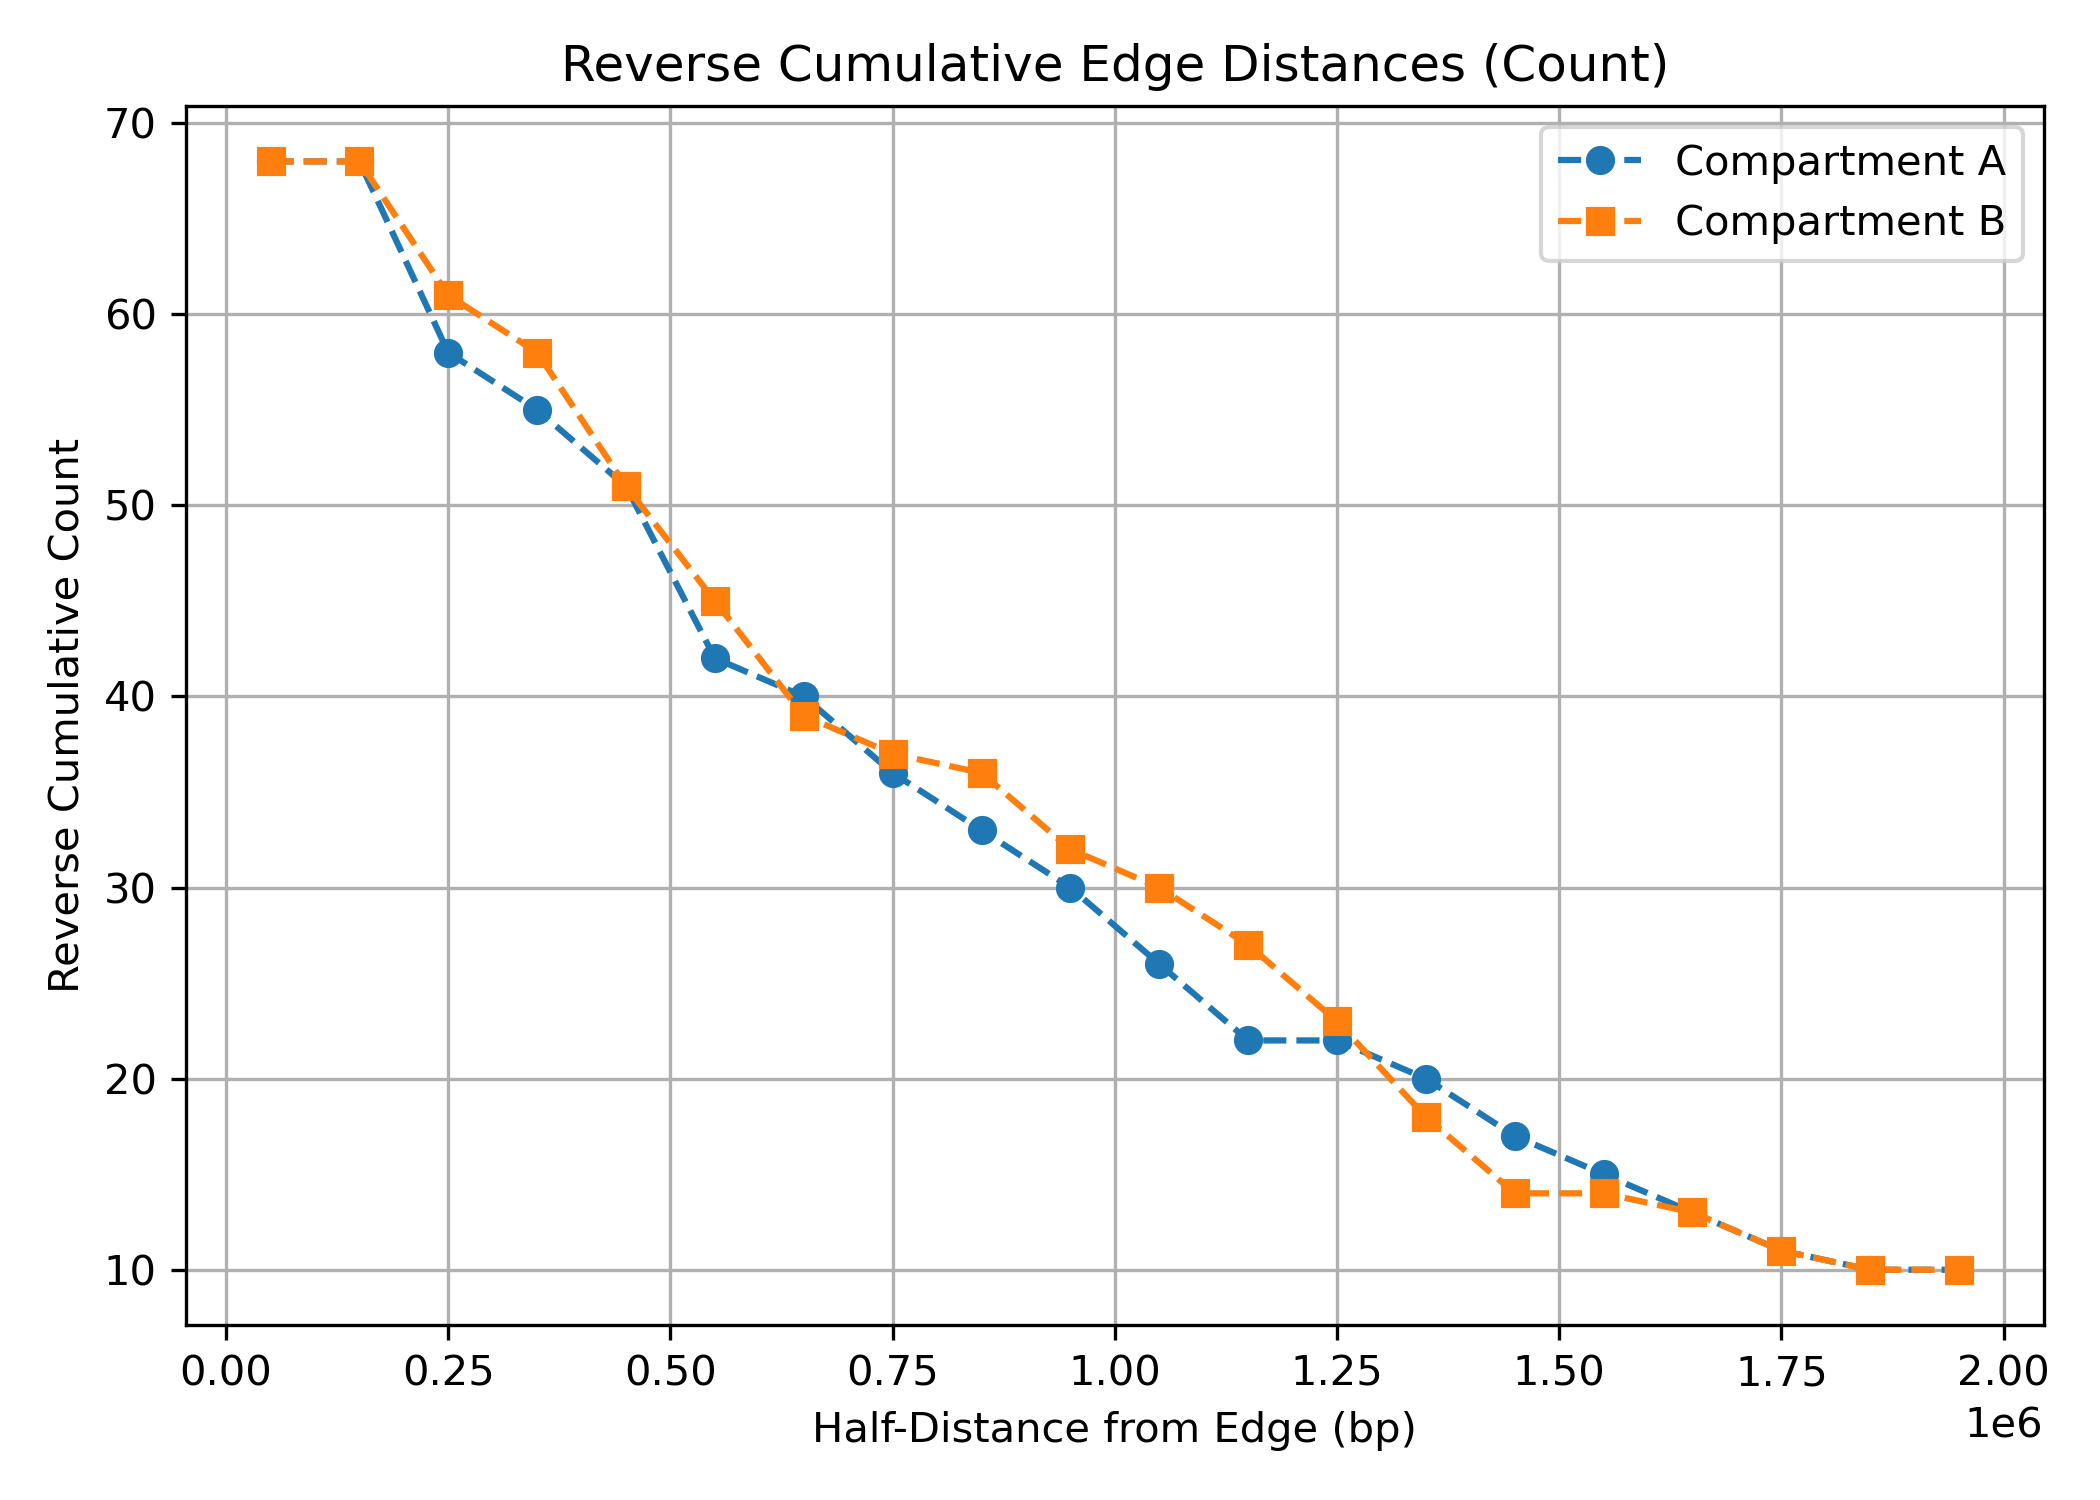
\includegraphics[width=1\linewidth,height=\textheight,keepaspectratio]{illustrations/reverse_cumulative_count_v2.png}

}

\caption{\label{fig-edge}Reverse cumulative counts of compartment edge
half-distances. Distances were calculated by first identifying
sequential transitions between compartments A and B (or B and A). For
each pair of transitions, the genomic distance between their start
positions was measured and halved, producing the ``half-distance''
metric. The reverse cumulative count at a given bin shows the number of
edges with half-distances greater than or equal to that bin's center,
representing the number of edges that could contribute data to
measurements at that spatial scale. Extending the plot to 2 Mb captures
the full range of half-distances observed.}

\end{figure}%

\chapter{compare GC conent to transition in
macaca}\label{compare-gc-conent-to-transition-in-macaca}

We compared GC content between A and B chromatin compartments for
chromosome 8 and chromosome X across five Macaca cell types:
fibroblasts, sperm, round spermatids, pachytene spermatocytes, and
spermatogonia. Chromatin compartments were defined from A--B and B--A
structural transitions, and GC content was measured separately for each
compartment.

For chromosome 8, the A compartment consistently showed higher GC
content than the B compartment in all cell types, which aligns with
expected genomic organization. In chromosome X, however, the differences
between compartments were smaller. In round spermatids, GC content was
nearly identical between A and B compartments, while in pachytene
spermatocytes, spermatogonia, and sperm, A and B compartments had
closely overlapping GC values. Interestingly, in fibroblasts the pattern
was reversed, with the B compartment displaying higher GC content than
the A compartment see Figure~\ref{fig-GC}.

\begin{figure}

\centering{

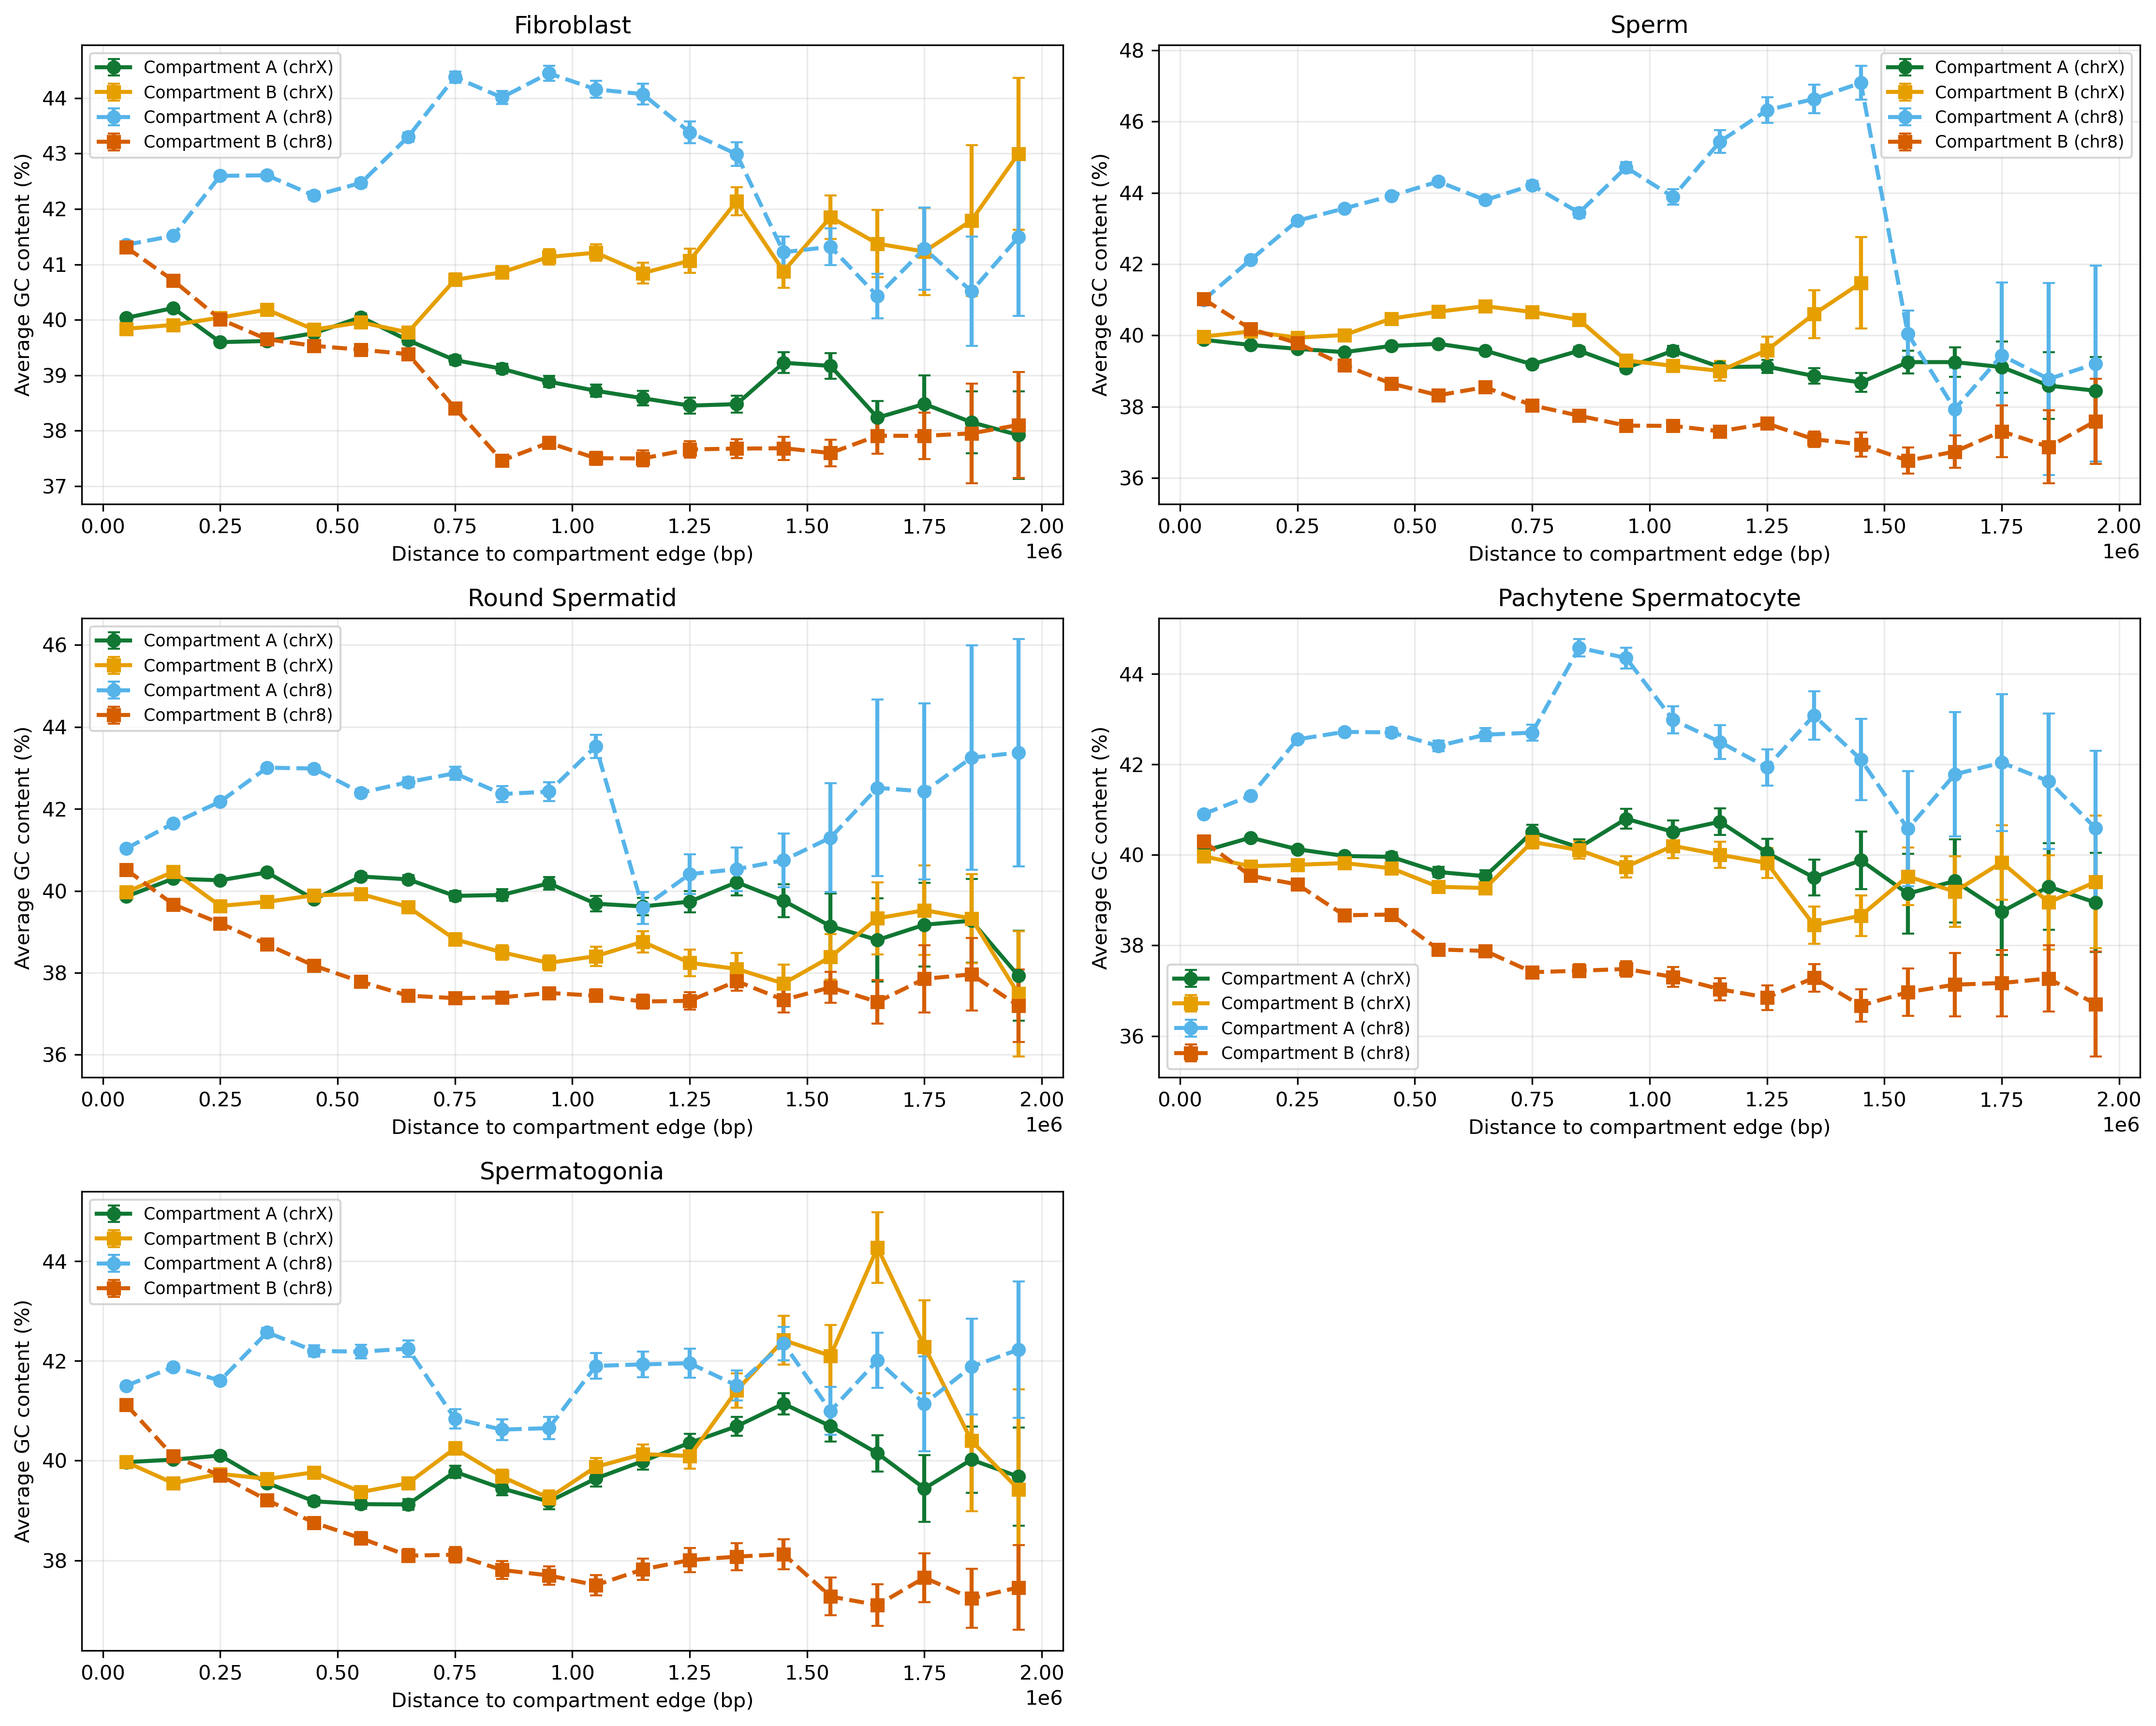
\includegraphics[width=1\linewidth,height=\textheight,keepaspectratio]{illustrations/gc_compartment_analysis_chrX_chr8_combined_20250812_144327.png}

}

\caption{\label{fig-GC}Compartment analysis for chromosomes X and 8 in
five Macaca cell types---fibroblasts, sperm, round spermatids, pachytene
spermatocytes, and spermatogonia. GC content was remapped to genomic
locations where chromatin structure transitions between compartments A
and B. The data were separated so that each compartment contains only A
or B structure. For each genomic bin, the plot shows the mean GC
content, with error bars representing the standard deviation of the
mean, adjusted by the effective edge contribution (accounting for how
many edges contribute at longer distances).For chromosome 8, the A
compartment exhibits higher GC content than the B compartment. In
tissues involved in spermatogenesis, chromosome X shows similar GC
content in both A and B compartments. In fibroblasts, GC content is
higher in the B compartment than in the A compartment.}

\end{figure}%

\chapter{CPG islands}\label{cpg-islands}

\begin{figure}

\centering{

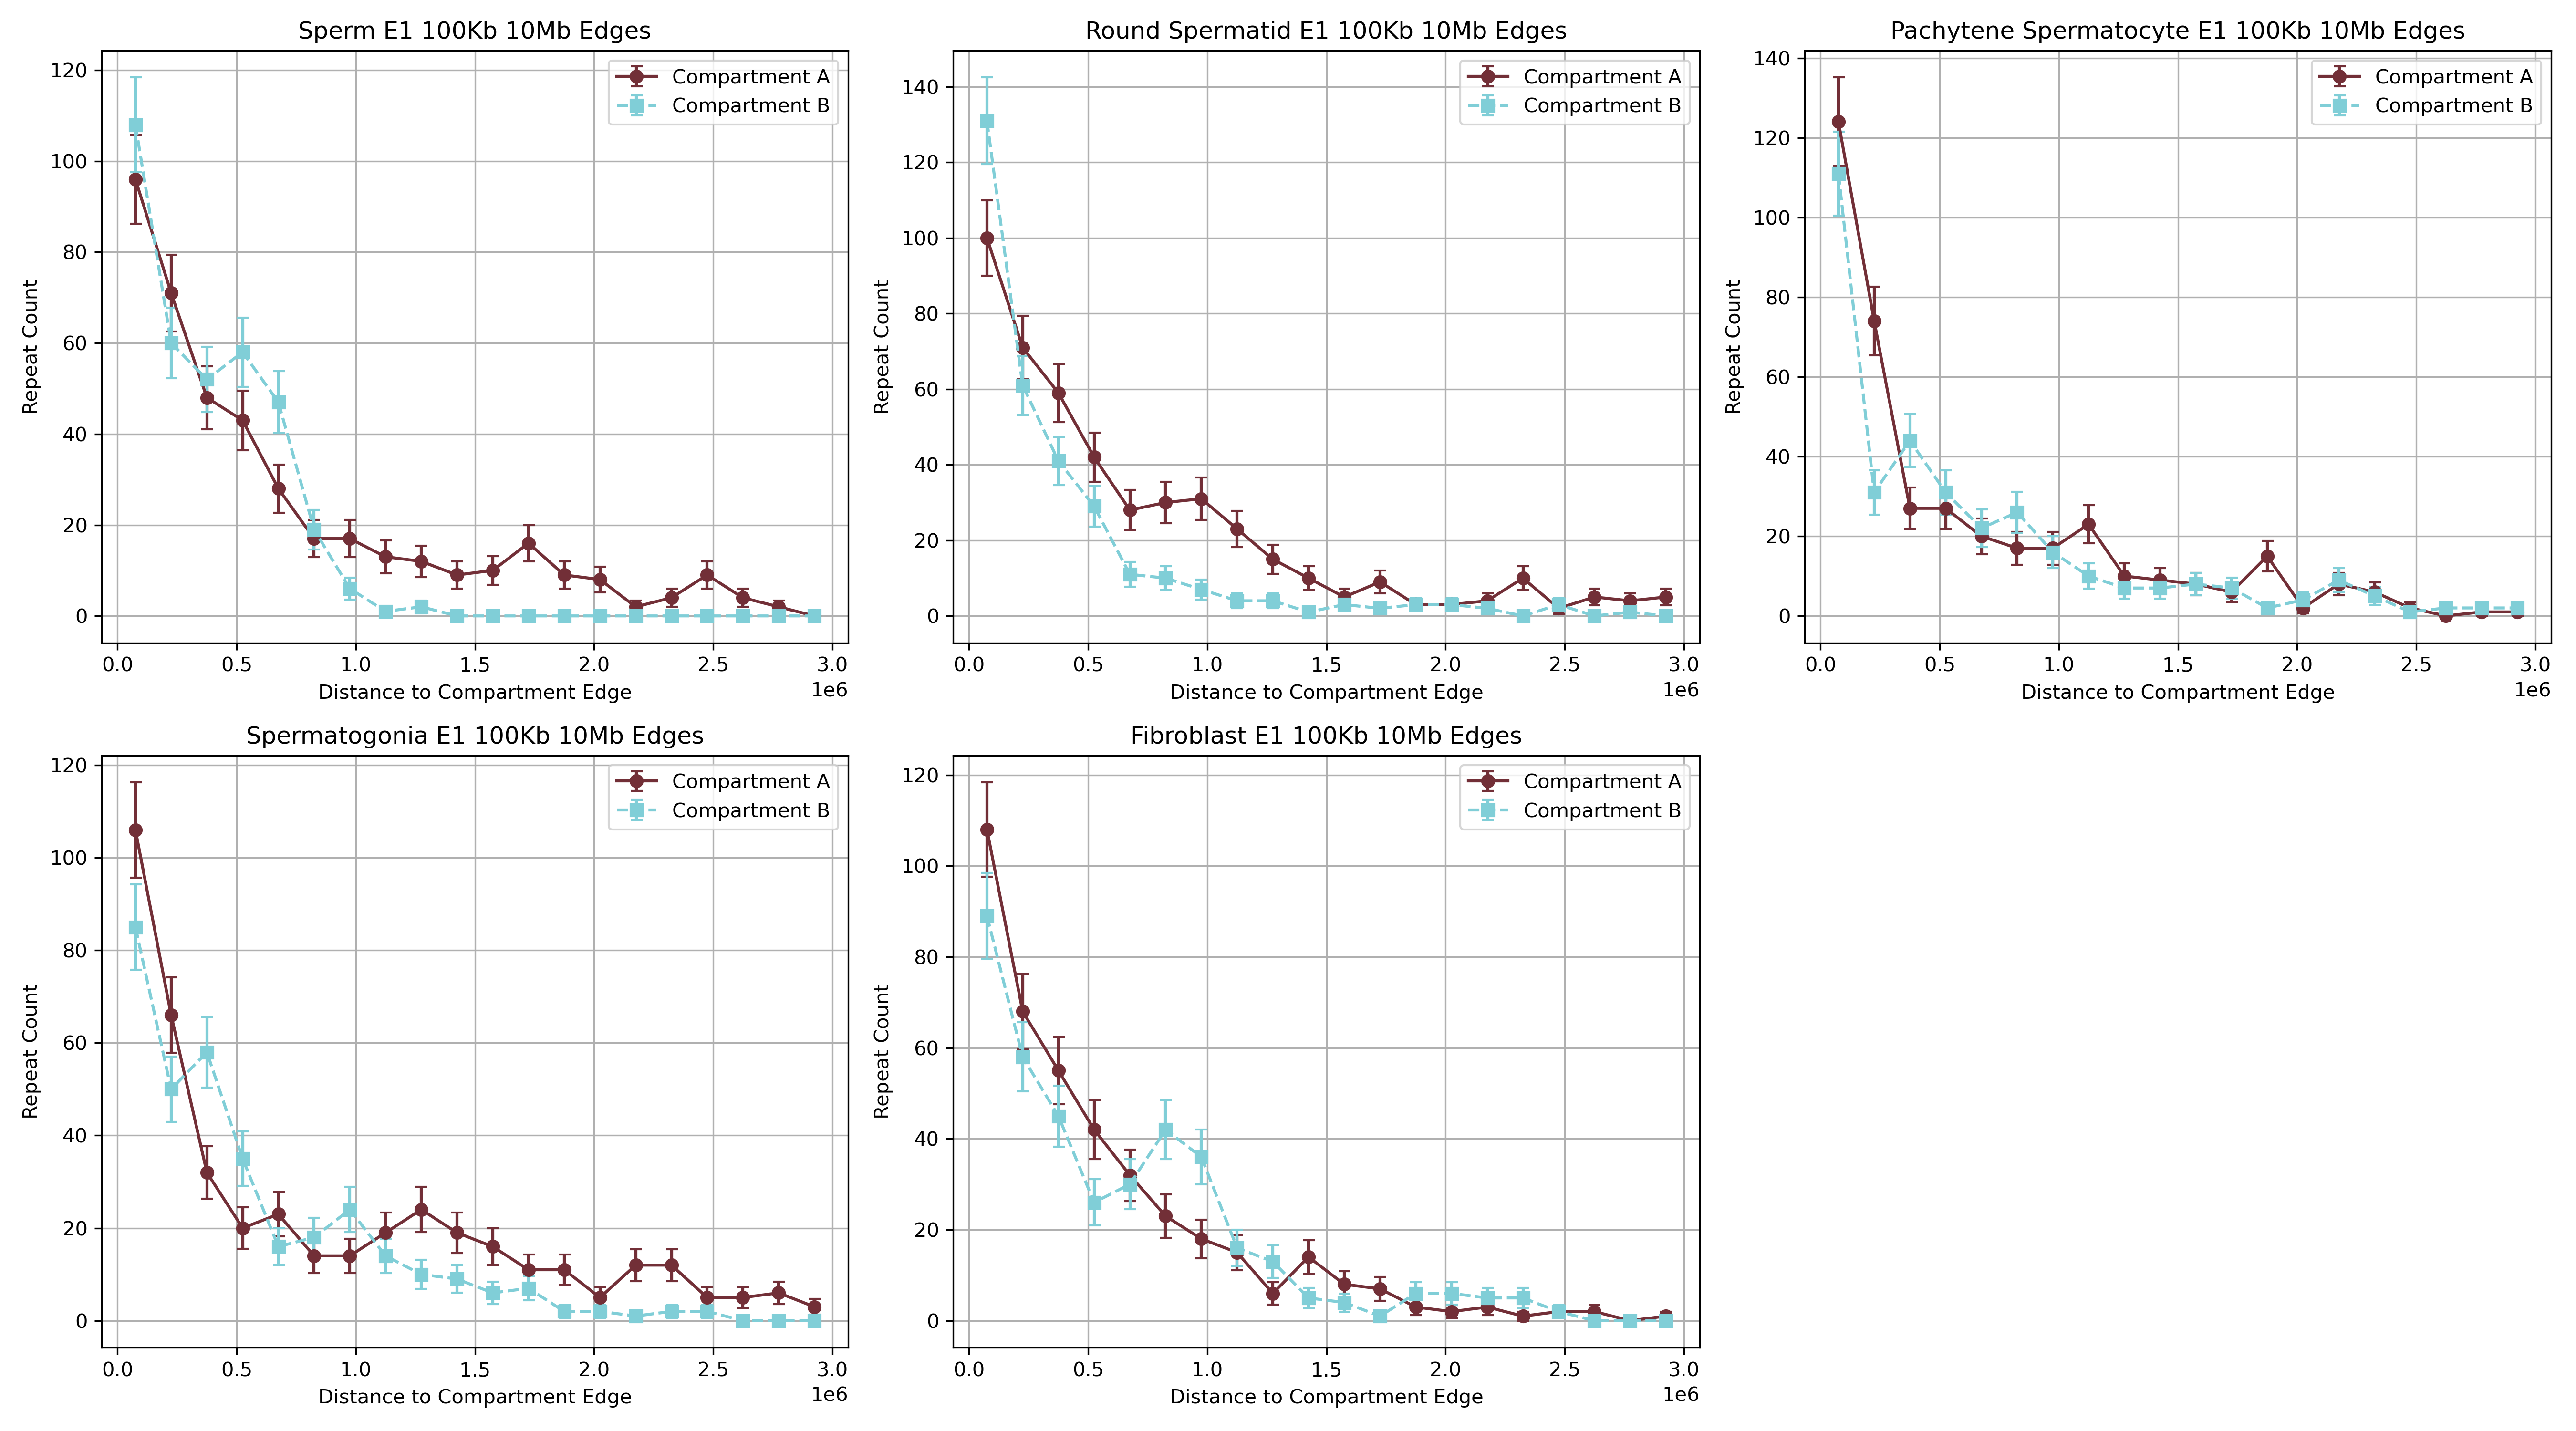
\includegraphics[width=1\linewidth,height=\textheight,keepaspectratio]{illustrations/CPG_islands_chrx_not_normalized.png}

}

\caption{\label{fig-CPG_not_normalized}}

\end{figure}%

\begin{figure}

\centering{

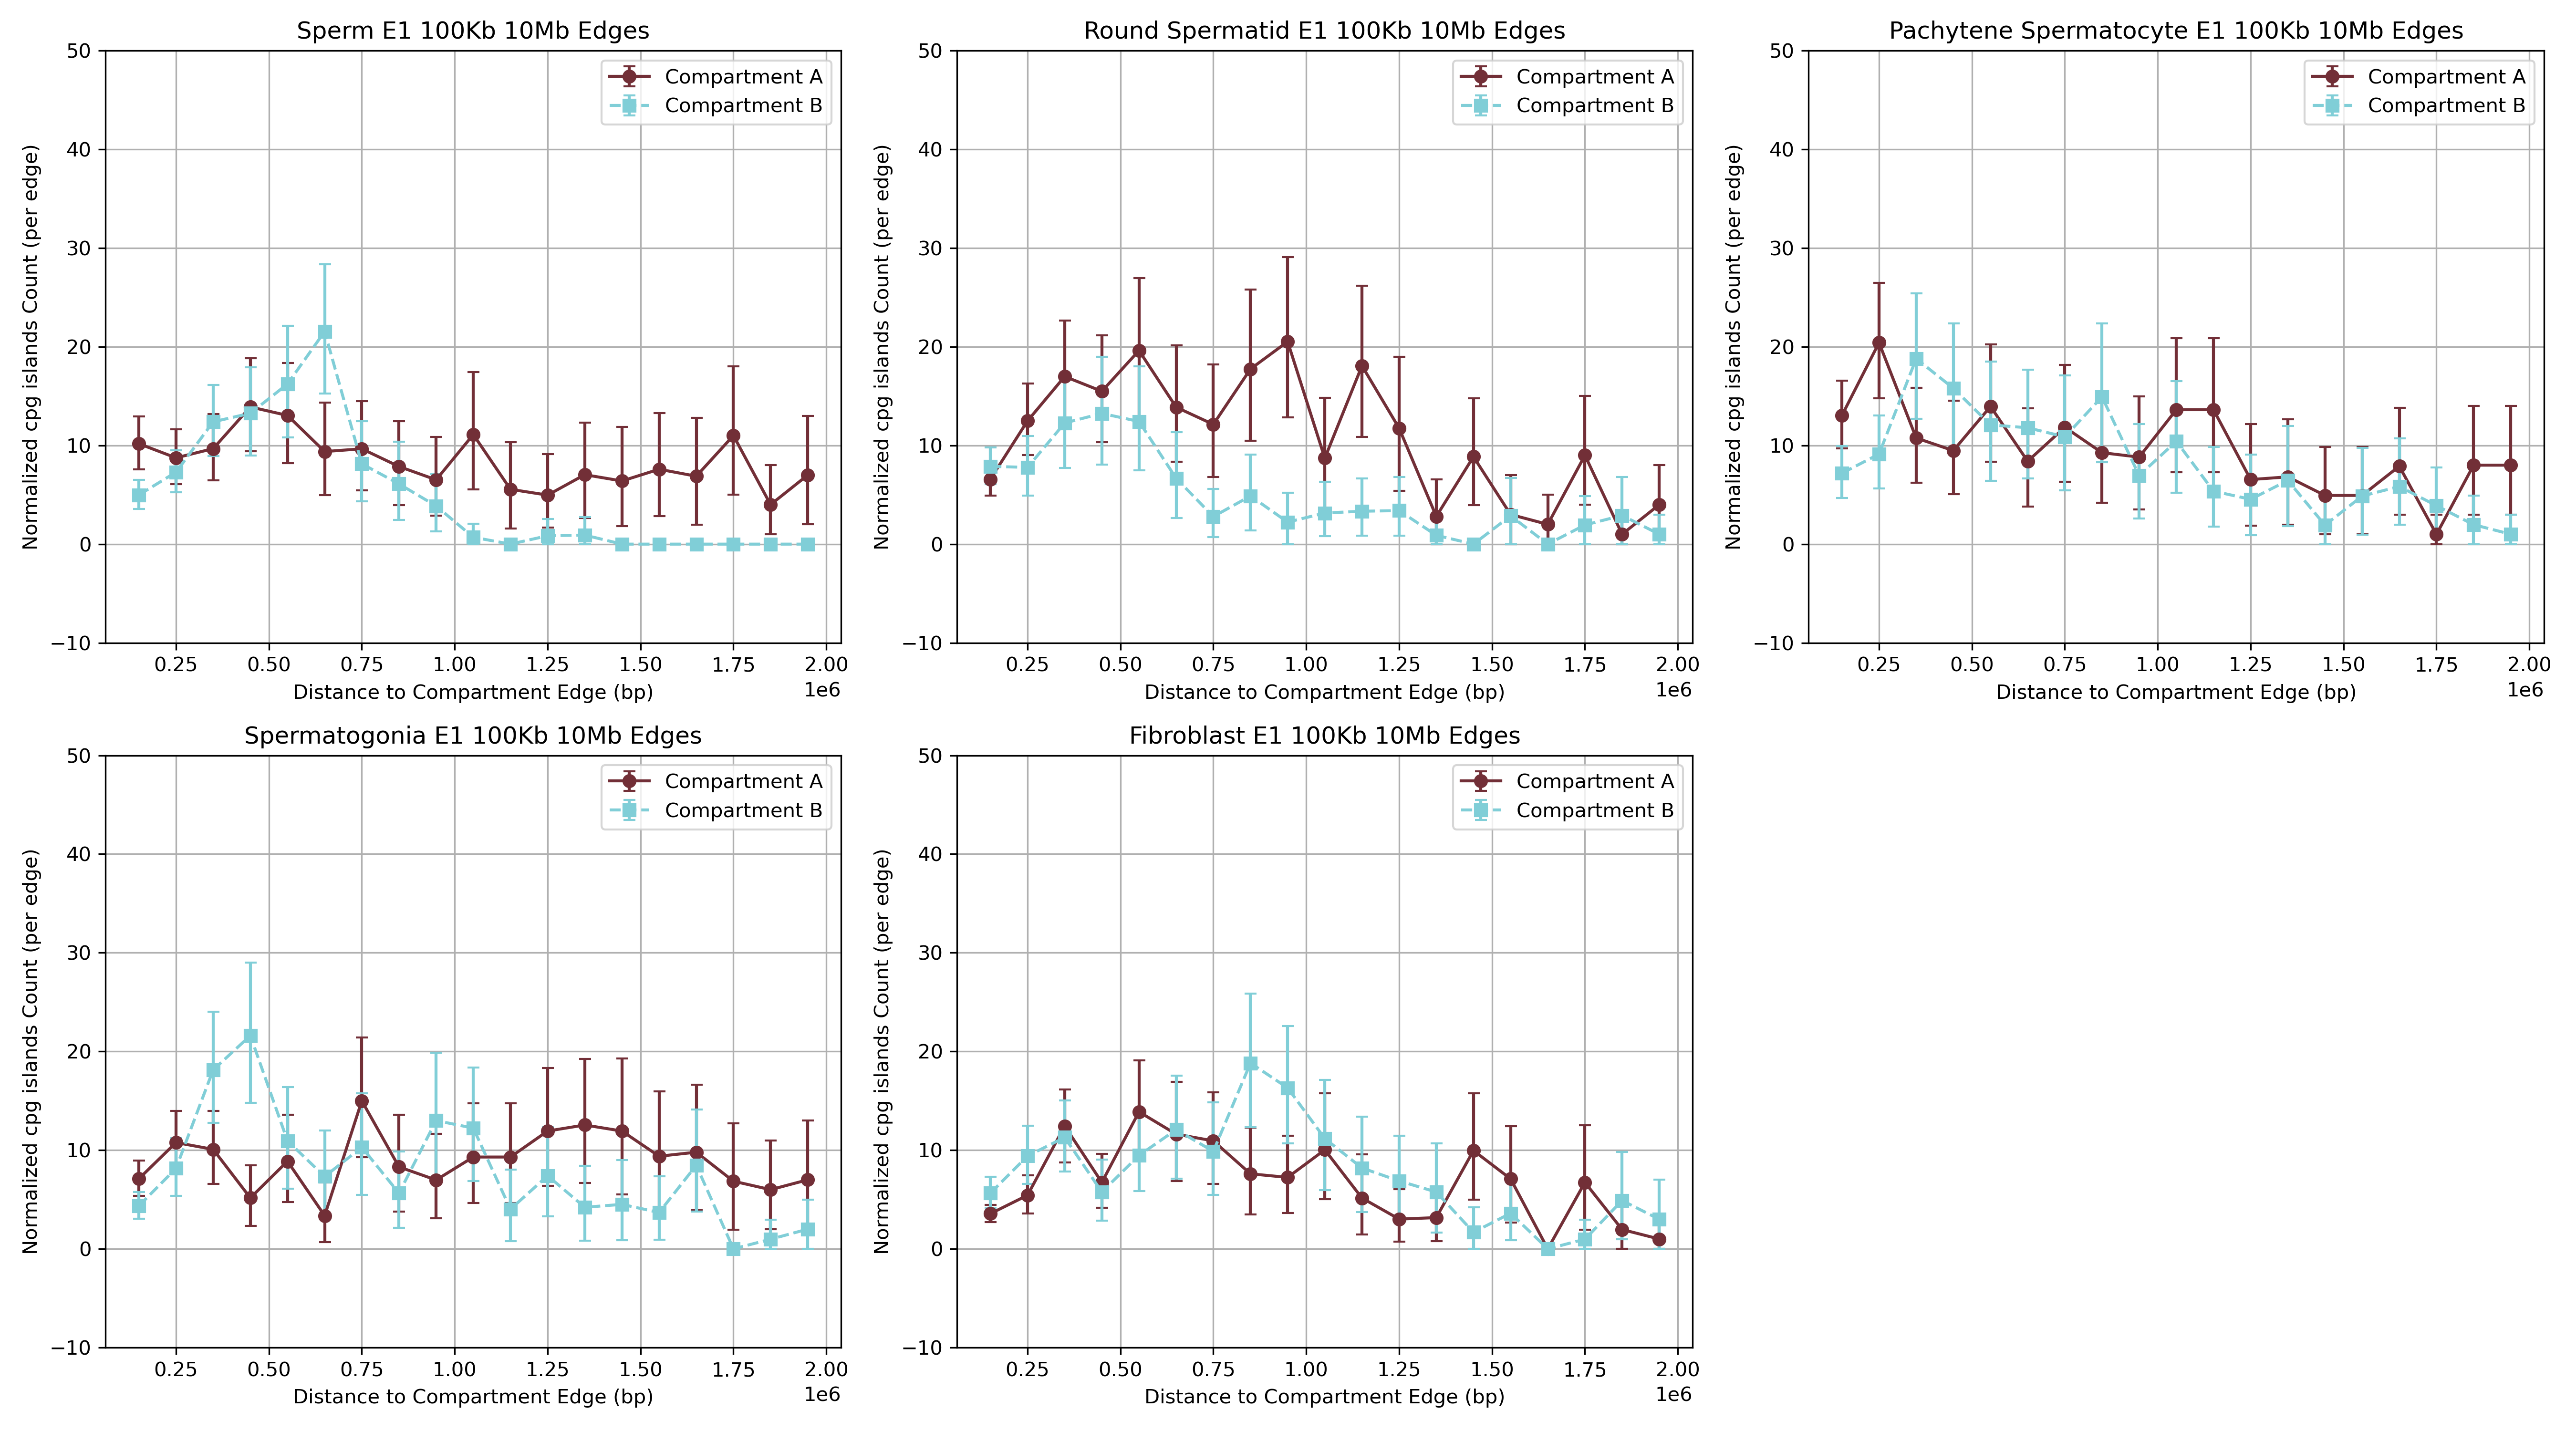
\includegraphics[width=1\linewidth,height=\textheight,keepaspectratio]{illustrations/CPG_islands_chrx_normalized_poisson_CI.png}

}

\caption{\label{fig-CPG_normalized}}

\end{figure}%

\begin{figure}

\centering{

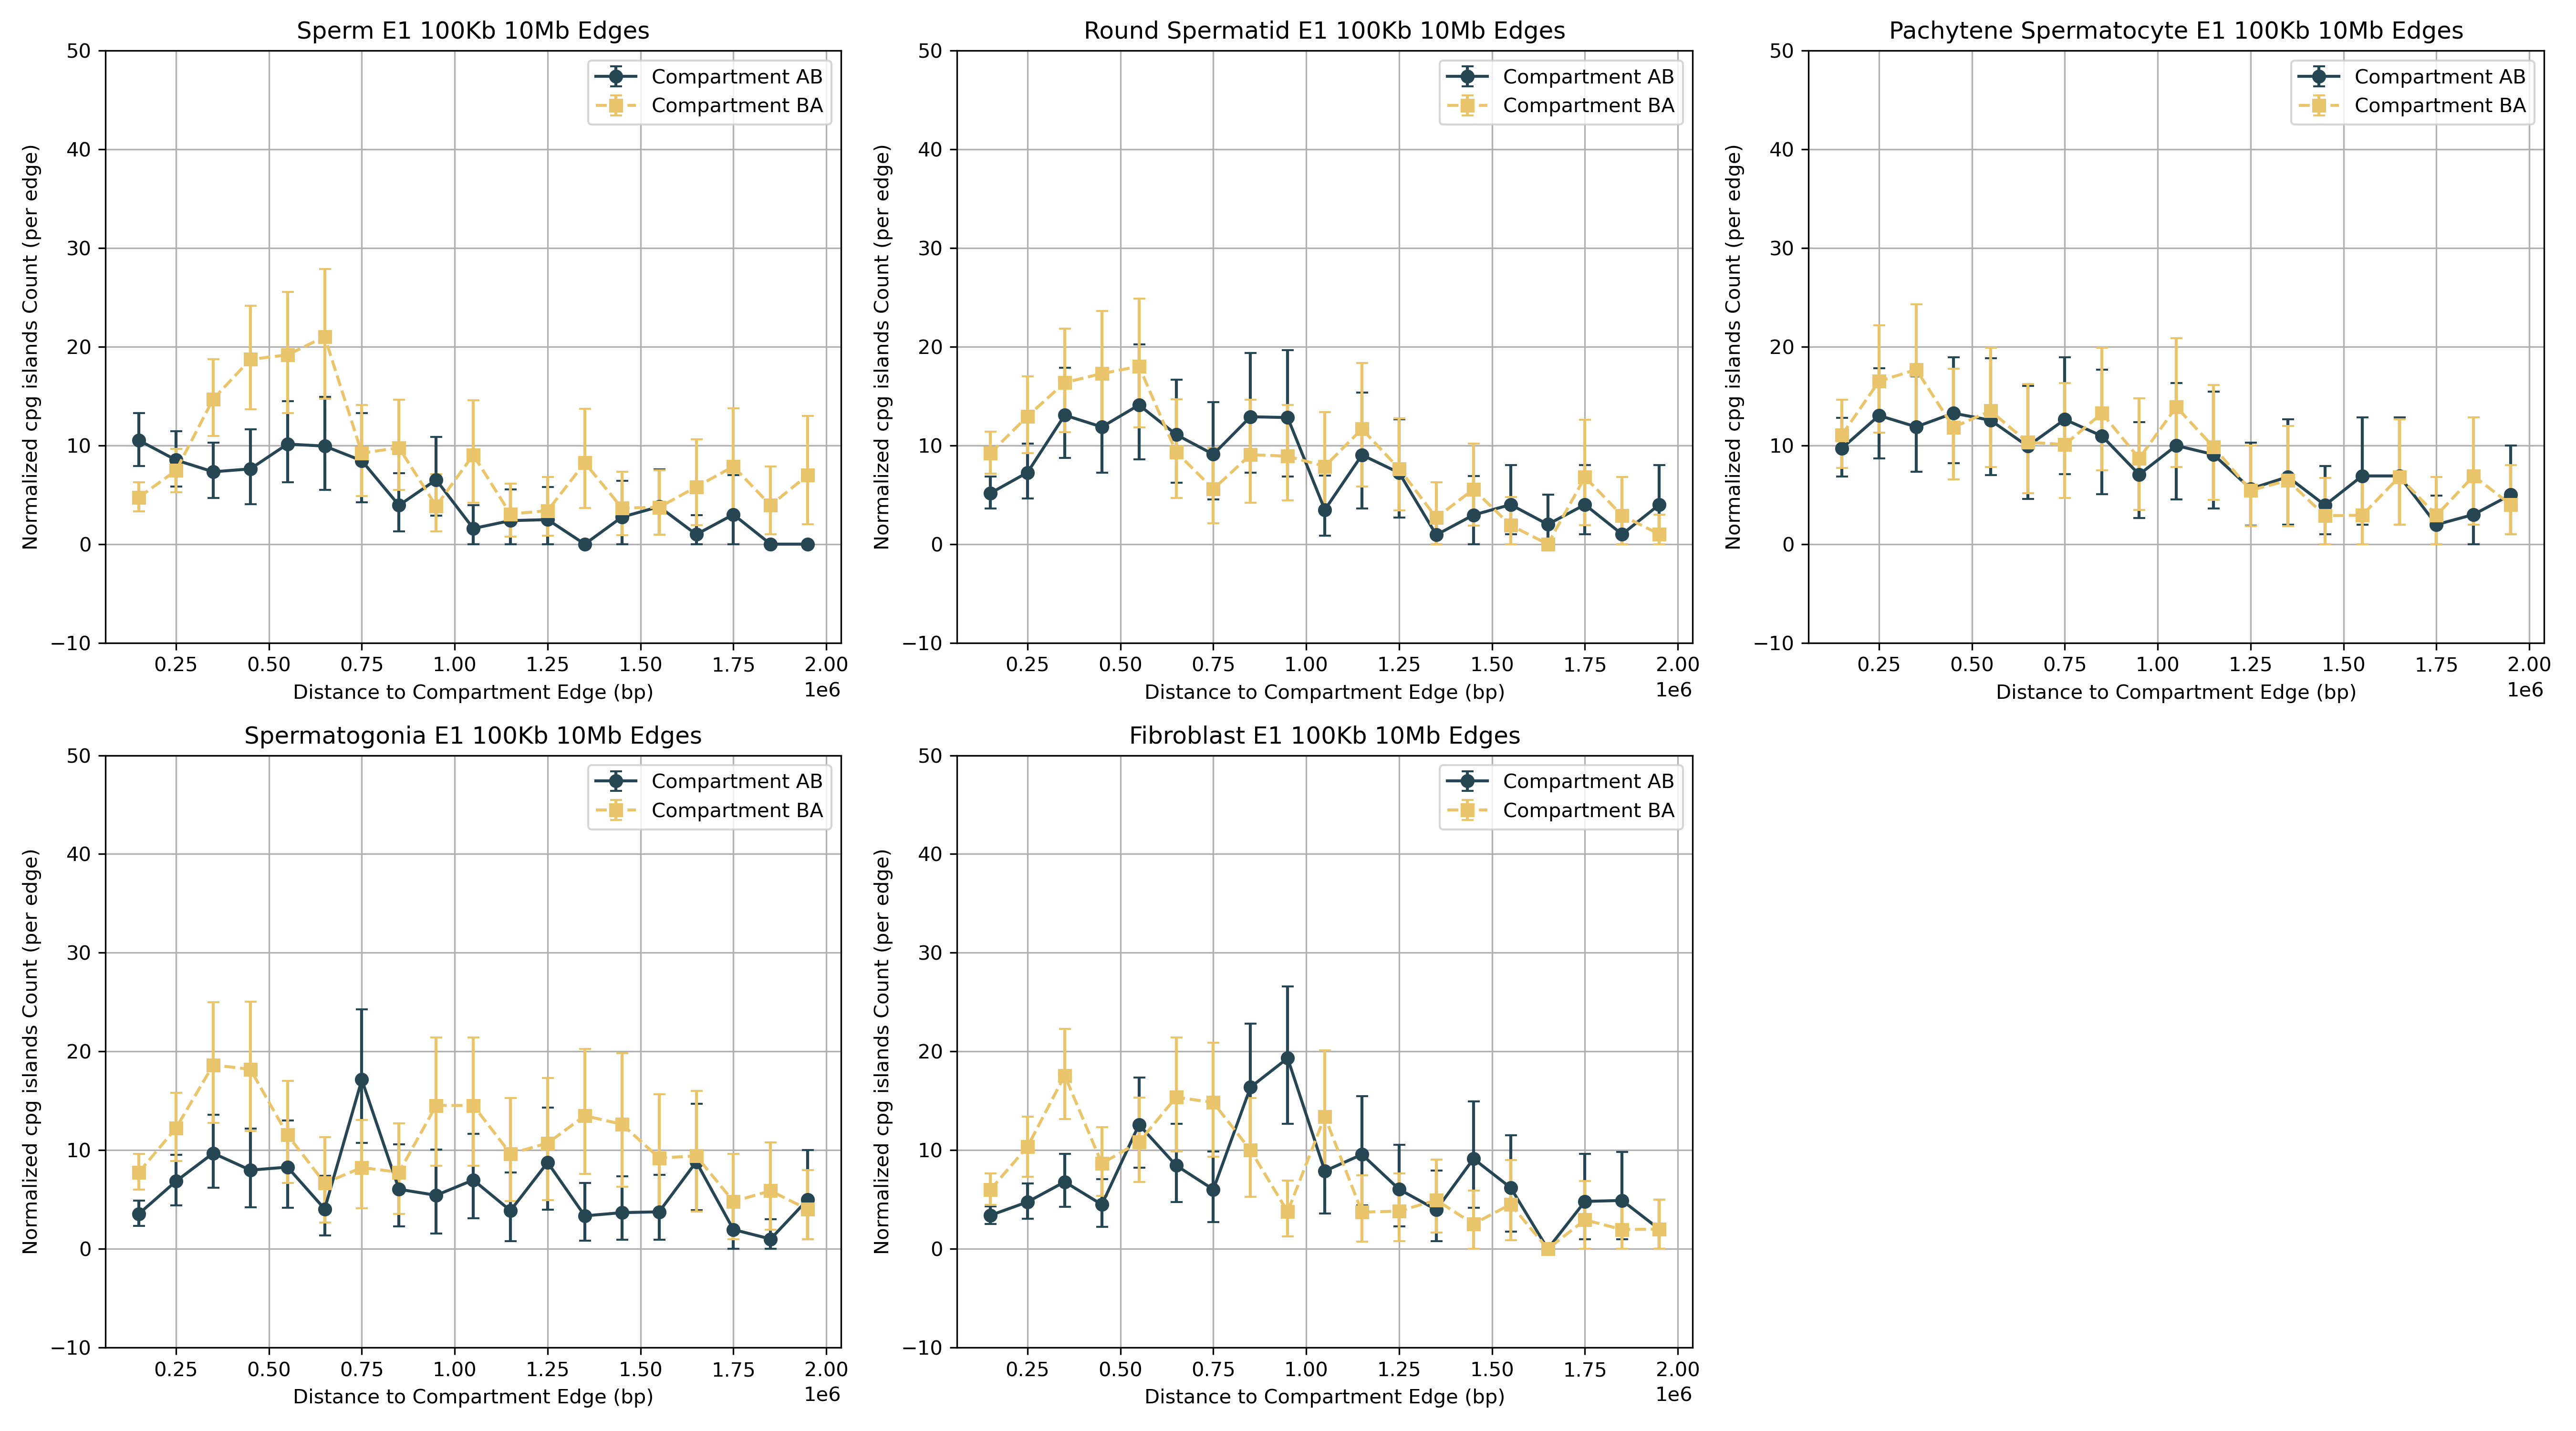
\includegraphics[width=1\linewidth,height=\textheight,keepaspectratio]{illustrations/CPG_islands_chrx_normalized_poisson_CI_AB_BA.png}

}

\caption{\label{fig-CPG_normalized}}

\end{figure}%

\section{chr 8}\label{chr-8}

\begin{figure}

\centering{

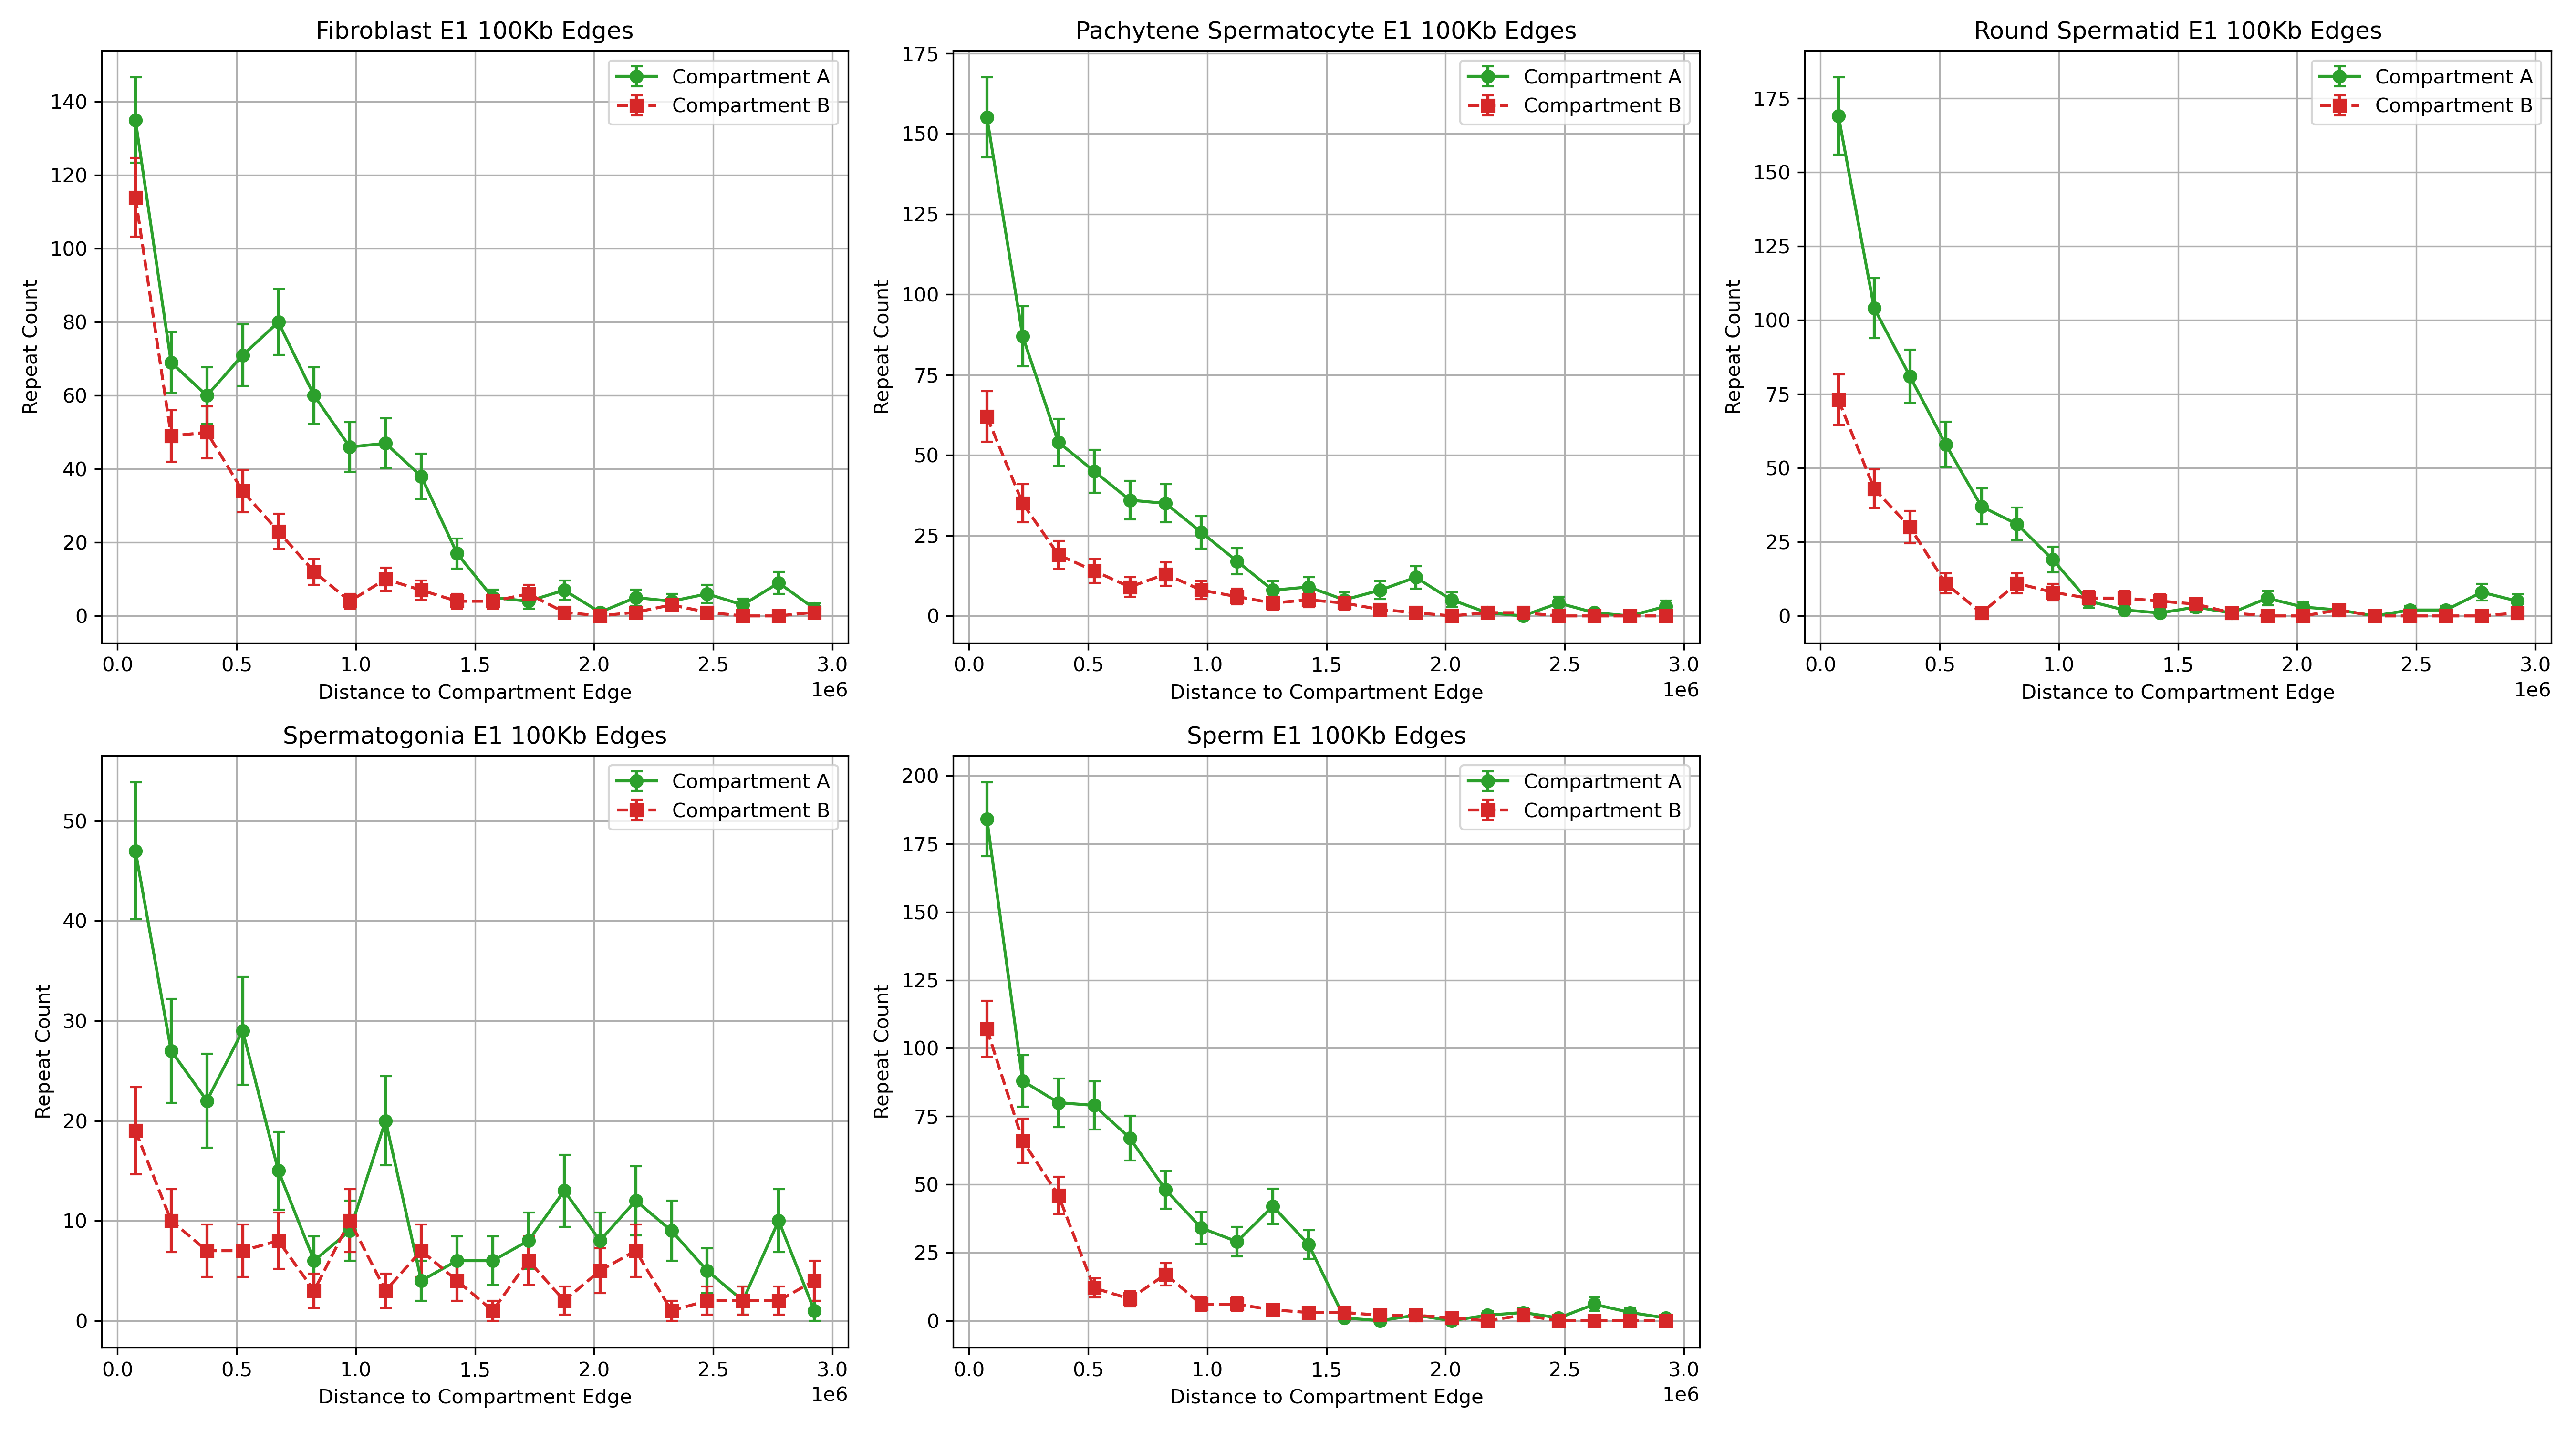
\includegraphics[width=1\linewidth,height=\textheight,keepaspectratio]{illustrations/CPG_islands_chr8_not_normalized.png}

}

\caption{\label{fig-CPG_not_normalized}}

\end{figure}%

\begin{figure}

\centering{

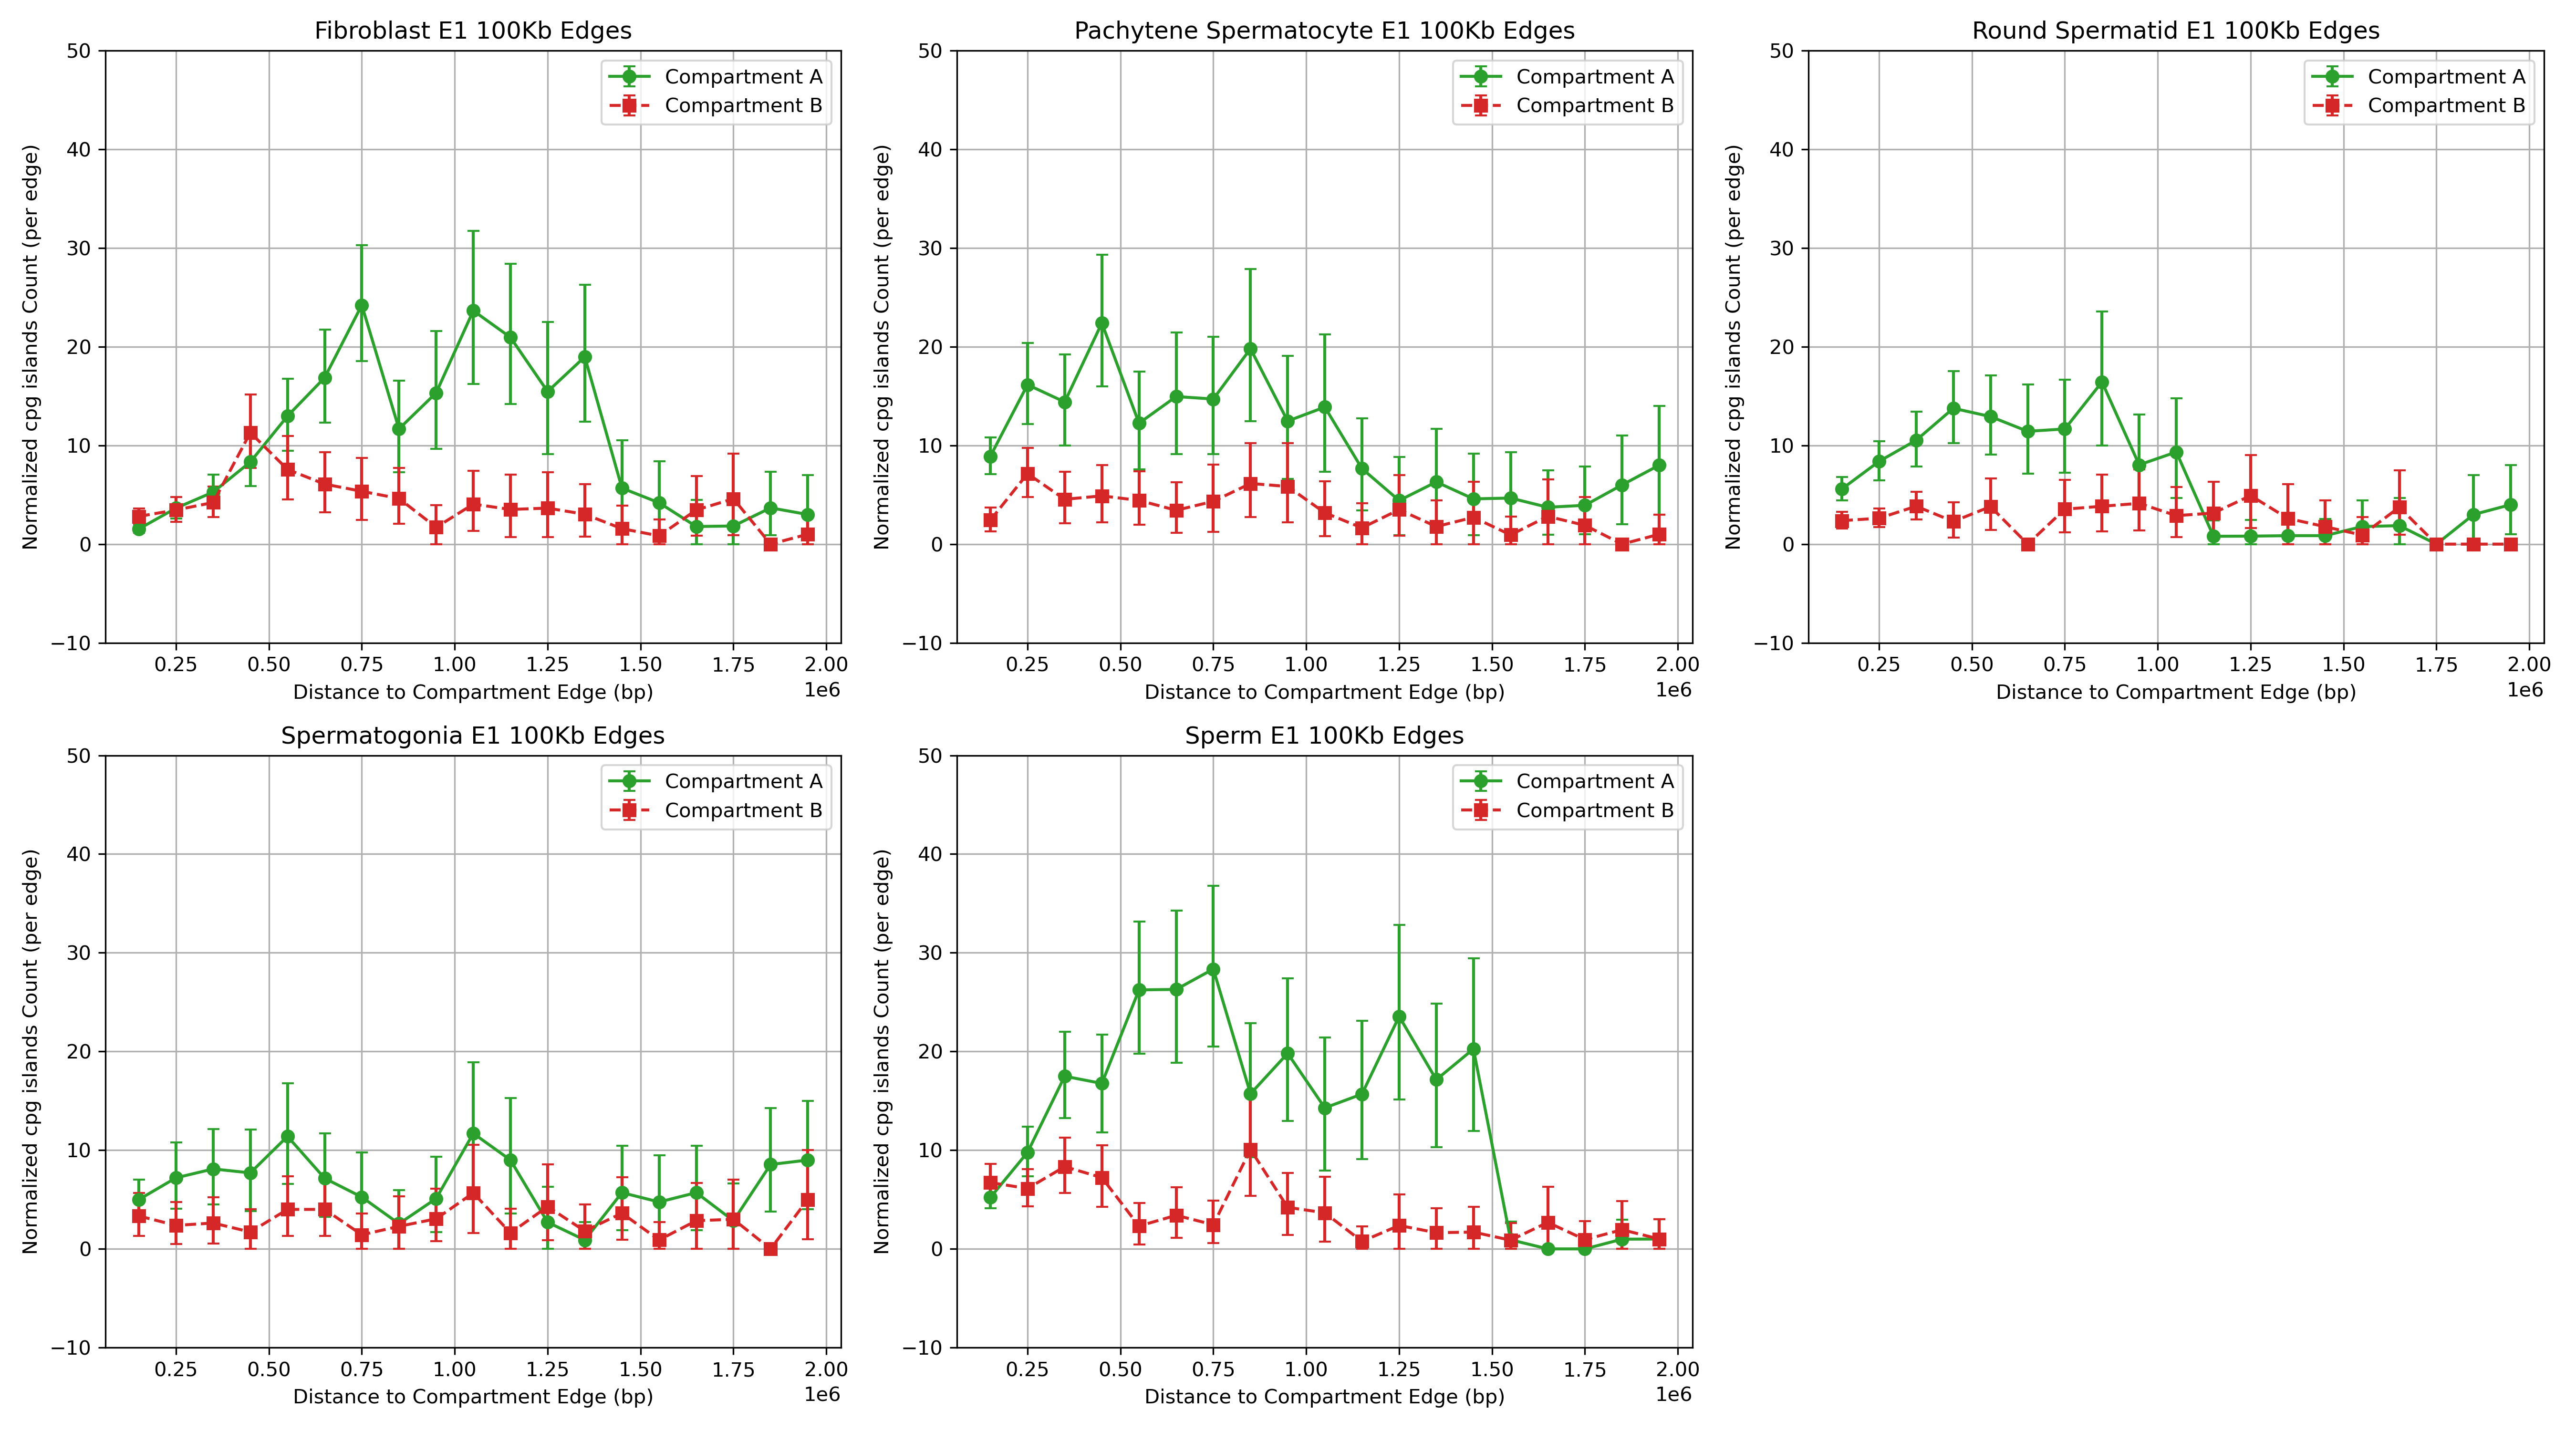
\includegraphics[width=1\linewidth,height=\textheight,keepaspectratio]{illustrations/CPG_islands_chr8_normalized_poisson_CI.png}

}

\caption{\label{fig-CPG_normalized}}

\end{figure}%

\begin{figure}

\centering{

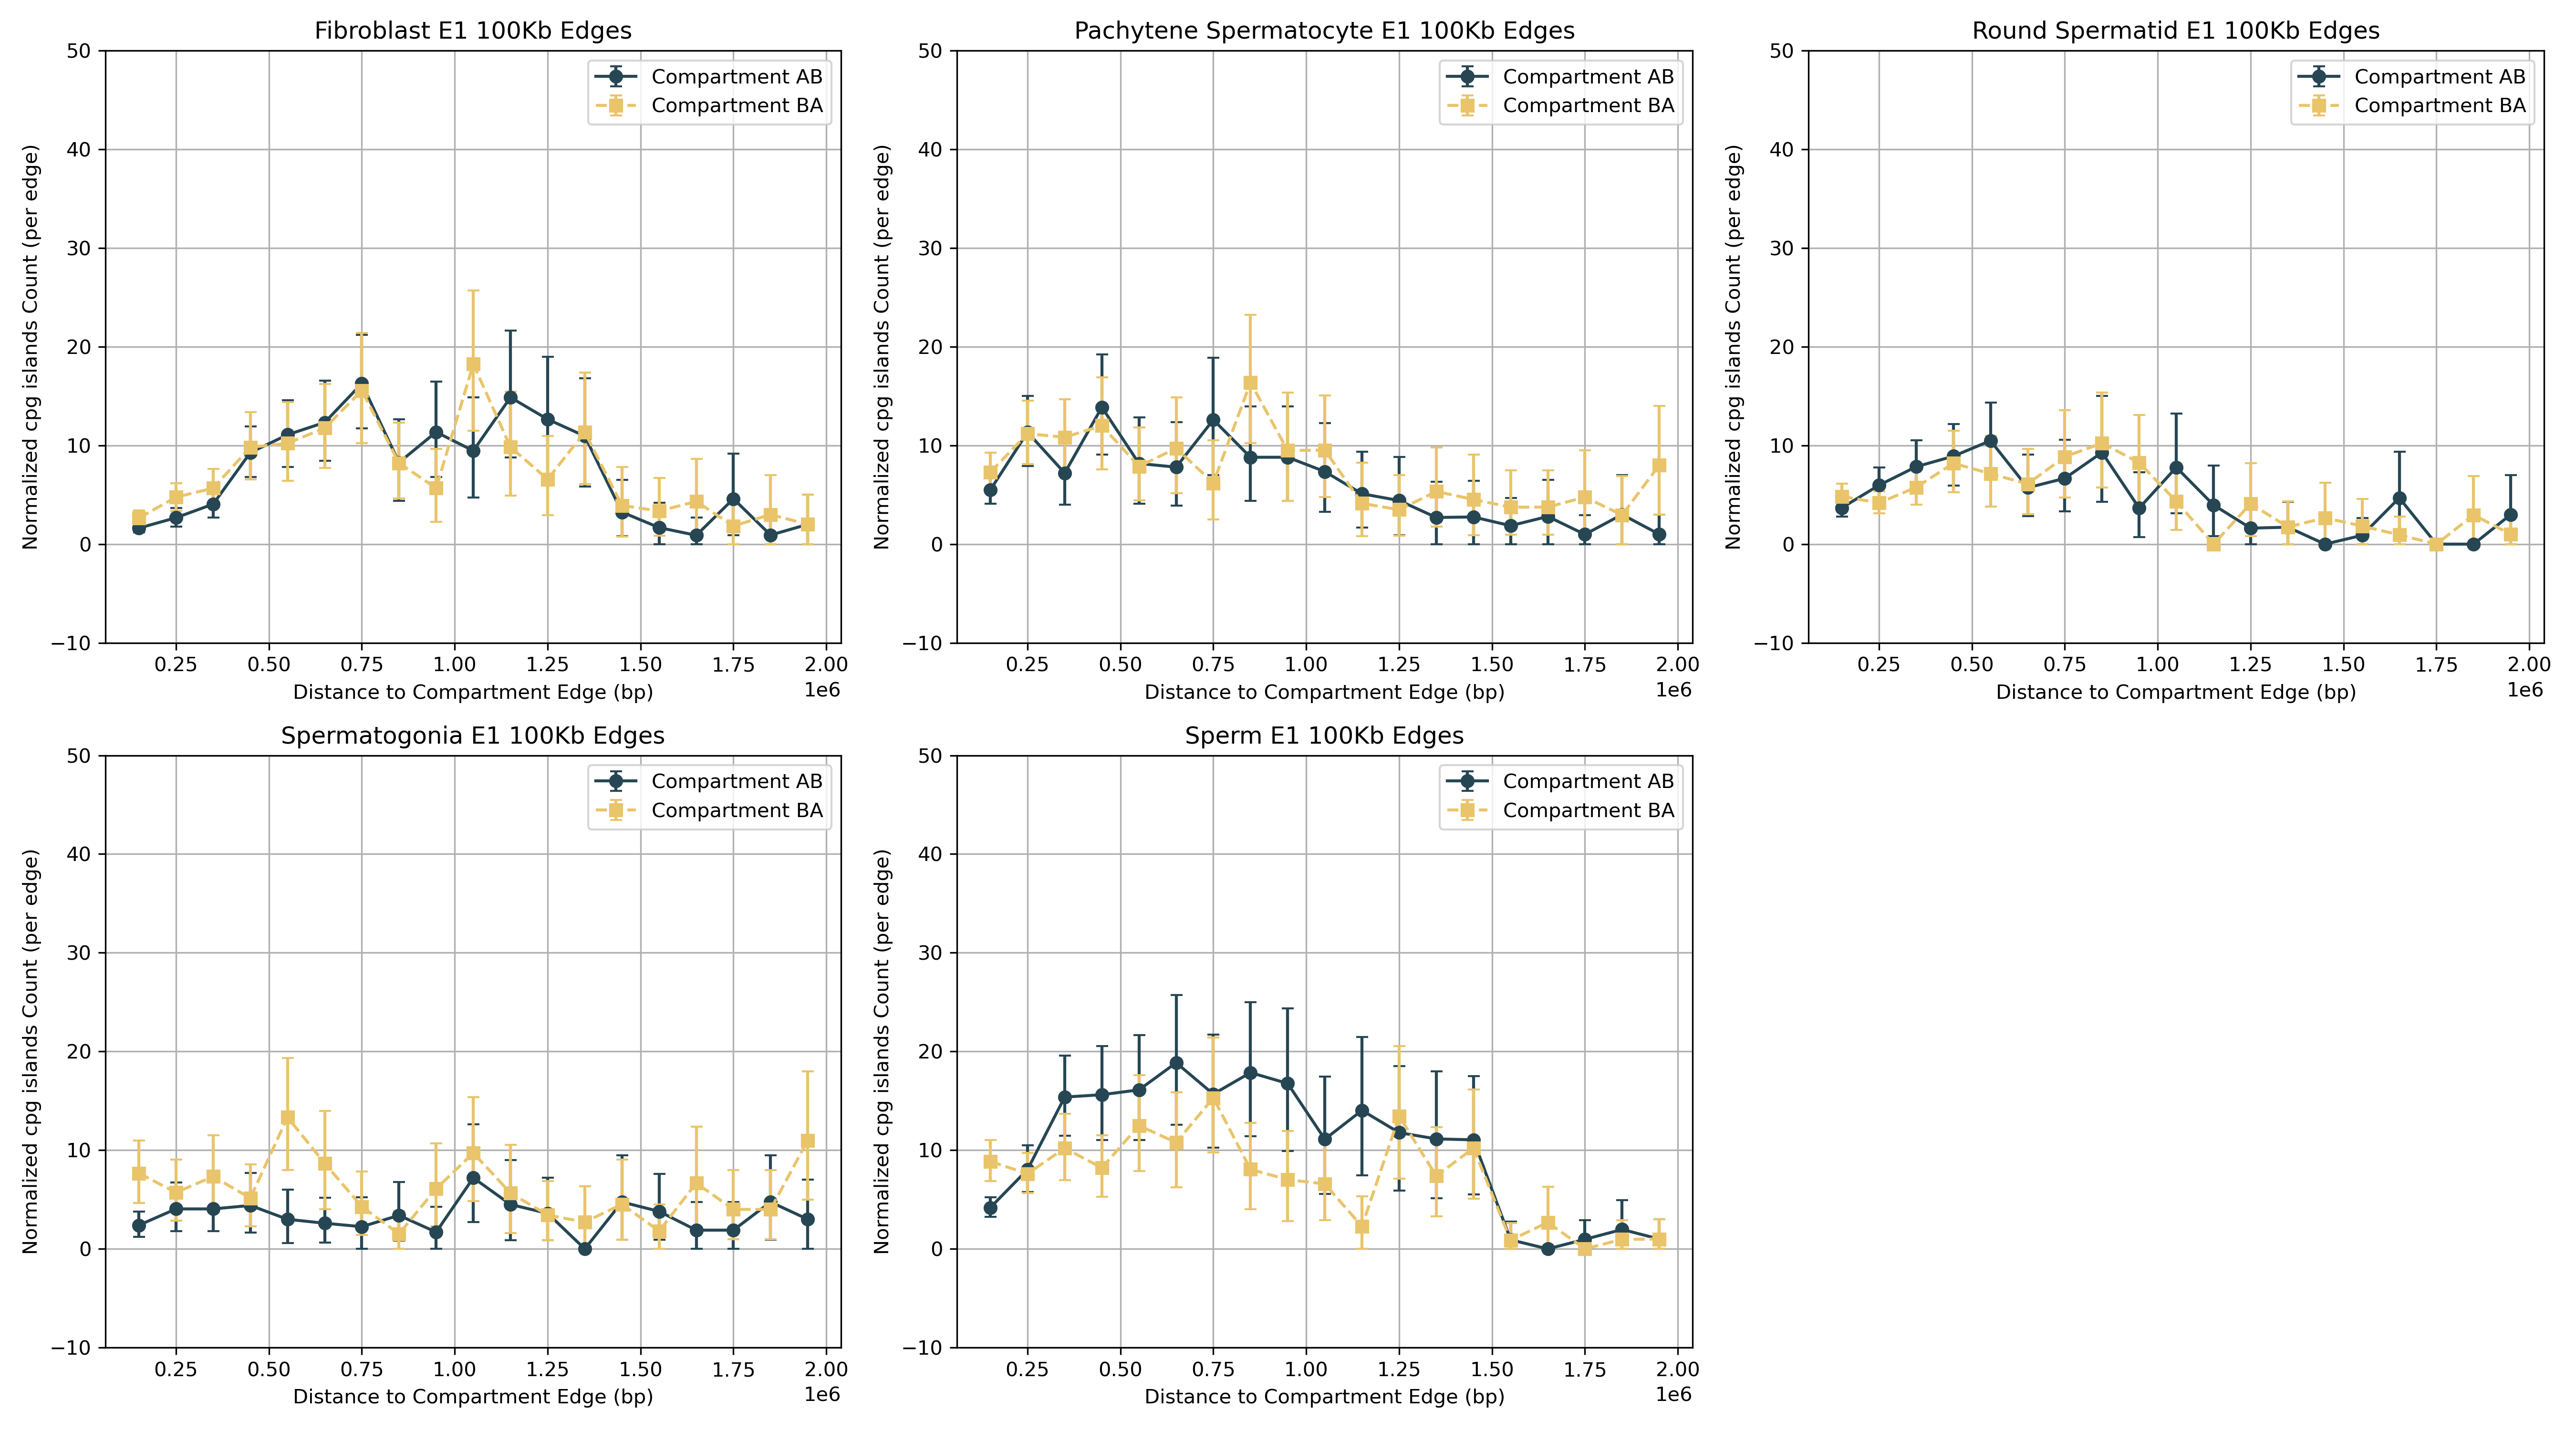
\includegraphics[width=1\linewidth,height=\textheight,keepaspectratio]{illustrations/CPG_islands_chr8_normalized_poisson_CI_AB_BA.png}

}

\caption{\label{fig-CPG_normalized}}

\end{figure}%

\chapter{repeat}\label{repeat}

\chapter{notes}\label{notes}

\chapter{cromatin structure and regulatiopn of
genes}\label{cromatin-structure-and-regulatiopn-of-genes}

\begin{enumerate}
\def\labelenumi{\arabic{enumi}.}
\setcounter{enumi}{1}
\tightlist
\item
  Regulation of Gene Expression The chromatin state influences gene
  accessibility:
\end{enumerate}

Open chromatin is associated with active gene transcription.

Closed chromatin represses gene activity. Repetitive elements near
regulatory genes can shift chromatin structure, acting as silencers or
enhancers depending on the epigenetic landscape (Venkatesh \& Workman,
2015).

Venkatesh \& Workman (2015) -- Histone exchange, chromatin structure and
transcription regulation Nature Reviews Molecular Cell Biology
Highlights the plasticity of chromatin around repeats and its impact on
transcription.

\chapter{repeats sorunding edges}\label{repeats-sorunding-edges}

\begin{enumerate}
\def\labelenumi{\arabic{enumi}.}
\tightlist
\item
  Genome Stability and Repression of Transposable Elements Repetitive
  sequences, such as LINEs, SINEs, and satellite DNA, are often silenced
  via heterochromatin formation. This closed chromatin state is
  essential to suppress transposable elements, which can otherwise
  mobilize and disrupt genome integrity (Moazed, 2011).
\end{enumerate}

Makova \& Hardison (2015) -- The effects of chromatin organization on
variation in mutation rates Nature Reviews Genetics Discusses how
heterochromatin protects repeats but also contributes to mutational
heterogeneity.

\begin{enumerate}
\def\labelenumi{\arabic{enumi}.}
\setcounter{enumi}{3}
\tightlist
\item
  Development and Cell Differentiation During development, regions with
  repetitive DNA undergo reconfiguration. The switch from euchromatin to
  heterochromatin is essential for cell lineage specification, and
  misregulation can cause developmental disorders (Gelato \& Fischle,
  2008).
\end{enumerate}

Ghosh \& Woodcock (2010) -- Chromatin higher-order structure and
dynamics Cold Spring Harbor Perspectives Explains how chromatin
compaction is governed by nucleosome positioning and repeat regions.

\subsection{Three-dimensional genome reorganization during mouse
spermatogenesis}\label{three-dimensional-genome-reorganization-during-mouse-spermatogenesis}

\begin{itemize}
\tightlist
\item
  Highlights how A/B compartment transitions coincide with major cell
  state transitions during spermatogenesis.
\item
  Found TF motifs and simple repeats enriched in switching regions.
\item
  Sheds light on regulatory elements linked to chromatin phase
  switching.
\end{itemize}

Core Findings This study investigates how the 3D organization of the
genome changes across seven sequential stages of mouse spermatogenesis,
using Hi-C technology. The work specifically focuses on topologically
associating domains (TADs), chromatin loops, and A/B compartments,
revealing highly dynamic reorganization events.

\begin{enumerate}
\def\labelenumi{\arabic{enumi}.}
\tightlist
\item
  TAD and Loop Dynamics Present in Type A spermatogonia (early stage).
\end{enumerate}

Disappear at pachytene stage (meiosis I prophase).

Reappear in mature spermatozoa.

This pattern indicates that TADs are not static during development and
may not be essential for transcription at all stages.

\begin{enumerate}
\def\labelenumi{\arabic{enumi}.}
\setcounter{enumi}{1}
\tightlist
\item
  CTCF Binding CTCF remains bound at TAD boundary regions even when TADs
  are absent (e.g., in pachytene spermatocytes).
\end{enumerate}

This suggests CTCF binding is not sufficient by itself to maintain 3D
structure.

\begin{enumerate}
\def\labelenumi{\arabic{enumi}.}
\setcounter{enumi}{2}
\tightlist
\item
  Enhancers, Promoters, and Active Transcription Despite the absence of
  TADs at pachytene, enhancers and promoters retain open chromatin.
\end{enumerate}

Transcription continues, implying that gene expression can occur
independently of higher-order chromatin loops.

\begin{enumerate}
\def\labelenumi{\arabic{enumi}.}
\setcounter{enumi}{3}
\tightlist
\item
  A/B Compartment Changes A/B compartments are largely conserved on
  autosomes throughout spermatogenesis.
\end{enumerate}

However, specific A -\textgreater{} B switching events are correlated
with changes in gene activity.

The X chromosome loses its A/B compartment structure during stages like
pachytene spermatocytes (pacSC), round spermatids (rST), and elongating
spermatids (eST).

Repeats and Chromatin Compartment Transitions TF motif enrichment was
analyzed in differentially active chromatin regions, which also included
repetitive DNA content.

During A/B compartment switching, particularly in regions transitioning
from B (closed) to A (open), some simple and low-complexity repeats were
enriched, suggesting a role in:

Regulatory rewiring during cell fate transition.

Chromatin accessibility and transcription activation.

The X chromosome, which undergoes massive reorganization and loss of A/B
compartment structure during specific stages (pacSC, rST, eST), may
exhibit a distinct repeat signature, though this was only briefly hinted
at in the paper.

(\textbf{article?})\{Luo2019, year = \{2019\}, title =
\{\{Three-dimensional genome reorganization during mouse
spermatogenesis\}\}, author = \{Luo, Zhen and Wang, Xin and Wang, Rui
and Chen, Jie and Chen, Yan and Xu, Qing and Cao, Jun\}, journal =
\{bioRxiv\}, doi = \{10.1101/585281\}, abstract = \{\{Dynamic changes in
chromatin architecture accompany spermatogenesis. Using Hi-C and
ATAC-seq, this study reveals A/B compartment transitions and
transcription factor motif enrichments that align with germ cell
stage-specific chromatin changes.\}\}, pages = \{\}, number = \{\},
volume = \{\}, pmid = \{\}, pmcid = \{\}, issn = \{\}, keywords = \{\},
local-url = \{https://www.biorxiv.org/content/10.1101/585281v1\} \}

\subsection{Single-cell long-read Hi-C,
scNanoHi-C2}\label{single-cell-long-read-hi-c-scnanohi-c2}

\begin{itemize}
\tightlist
\item
  Uses single-cell Hi-C to resolve chromatin changes in early germ
  cells.
\item
  Finds TE subfamilies enriched differently in A/B compartments,
  suggesting a regulatory function of repeat elements.
\end{itemize}

Key Findings Summary Development of scNanoHi-C2

The authors introduce scNanoHi-C2, a novel single-cell long-read Hi-C
technique.

It overcomes limitations of standard Hi-C by capturing long-range,
multi-contact chromatin interactions in individual cells.

3D Genome Dynamics in Germ Cells

Applied to embryonic germline cells, the technique reveals:

Stage-specific topological reorganization of the genome.

Highly dynamic A/B compartment transitions, even at early embryonic
stages.

Repeat Element Profiling

The study shows distinct enrichment patterns of transposable elements
(TEs) in A and B compartments.

LINEs and SINEs were differentially represented, correlating with
developmental chromatin remodeling.

These repeats may contribute to insulation, compartmental identity, or
nuclear architecture.

Chromatin Rewiring during Primordial Germ Cell (PGC) Development

Early embryonic germ cells exhibit weaker TAD boundaries and less stable
compartments compared to somatic cells.

As differentiation progresses, compartment strength increases,
indicating a progressive maturation of 3D genome organization.

X Chromosome Inactivation Patterns

The paper provides high-resolution views of X chromosome organization,
noting changes in compartmental asymmetry and pairing during early germ
cell development.

(\textbf{article?})\{Lu2025, year = \{2025\}, title = \{\{Single-cell
long-read Hi-C, scNanoHi-C2, details 3D genome reorganization in
embryonic-stage germ cells\}\}, author = \{Lu, Jiawei and Li, Wen and
Tang, Fuchou\}, journal = \{Nature Structural \& Molecular Biology\},
doi = \{10.1038/s41594-025-01604-7\}, issn = \{1545-9985\}, abstract =
\{\{This study applies scNanoHi-C2 to reveal high-resolution single-cell
3D chromatin structure changes during germline development. Transposable
elements and repeat families were differentially enriched in A/B
compartments, impacting developmental regulation.\}\}, pages = \{\},
number = \{\}, volume = \{\}, pmid = \{\}, pmcid = \{\}, keywords =
\{\}, local-url = \{https://www.nature.com/articles/s41594-025-01604-7\}
\}

\subsection{3D genome remodeling and homologous pairing during meiotic
prophase}\label{d-genome-remodeling-and-homologous-pairing-during-meiotic-prophase}

\begin{itemize}
\tightlist
\item
  Simple and LINE repeats enriched in B compartments, involved in
  meiotic structural integrity.
\end{itemize}

Key Findings Summary This study integrates Hi-C chromatin conformation
capture with super-resolution microscopy to uncover how 3D genome
architecture is remodeled during meiotic prophase I in both male and
female germlines (spermatogenesis and oogenesis) in mice.

Homologous Chromosome Pairing Chromosomes exhibit precise and
progressive pairing during prophase I.

The study captures early pairing events in spermatocytes and oocytes,
using high-resolution contact maps.

Contact frequency increases significantly in homologous regions during
zygotene and pachytene stages.

\begin{enumerate}
\def\labelenumi{\arabic{enumi}.}
\setcounter{enumi}{1}
\tightlist
\item
  Chromatin Compartment Remodeling A/B compartments are weakened or
  restructured during prophase.
\end{enumerate}

Specific B compartments, enriched in LINE elements and heterochromatin,
show elevated pairing dynamics.

Suggests B compartment flexibility supports pairing more than A.

\begin{enumerate}
\def\labelenumi{\arabic{enumi}.}
\setcounter{enumi}{2}
\tightlist
\item
  Role of Repeat Elements Repeat-rich regions, especially LINEs and
  LTRs, are preferentially localized to B compartments and correlate
  with stronger interhomolog interactions.
\end{enumerate}

Repeats may play a structural role in mediating nuclear architecture
during meiosis.

\begin{enumerate}
\def\labelenumi{\arabic{enumi}.}
\setcounter{enumi}{3}
\tightlist
\item
  Sex Differences in Chromosome Pairing The authors find distinct
  dynamics between male and female germ cells, including:
\end{enumerate}

Differences in compartment switching speed.

Asynchronous timing in homolog pairing progression.

Oocytes retain more stable open chromatin than spermatocytes during
mid-prophase.

(\textbf{article?})\{He2023, year = \{2023\}, title = \{\{3D genome
remodeling and homologous pairing during meiotic prophase of mouse
oogenesis and spermatogenesis\}\}, author = \{He, Jianrong and Yan, Ao
and Chen, Bohan and Huang, Jin and Kee, Kehkooi\}, journal =
\{Developmental Cell\}, doi = \{10.1016/j.devcel.2023.07.004\}, issn =
\{1534-5807\}, abstract = \{\{By applying Hi-C and super-resolution
microscopy, this study tracks chromatin compartment transitions and
homolog pairing in meiosis. Repeat-enriched B compartments show
increased pairing dynamics and regulate meiotic architecture.\}\}, pages
= \{\}, number = \{\}, volume = \{\}, pmid = \{\}, pmcid = \{\},
keywords = \{\}, local-url =
\{https://www.cell.com/developmental-cell/abstract/S1534-5807(23)00553-1\}
\}

\subsection{DICER regulates repeat RNA and chromosome segregation
(maybe???)}\label{dicer-regulates-repeat-rna-and-chromosome-segregation-maybe}

\begin{itemize}
\tightlist
\item
  Satellite repeats involved in chromatin architecture, A/B compartment
  boundary insulation via RNA-based silencing pathways.
\end{itemize}

(\textbf{article?})\{He2023, year = \{2023\}, title = \{\{3D genome
remodeling and homologous pairing during meiotic prophase of mouse
oogenesis and spermatogenesis\}\}, author = \{He, Jianrong and Yan, Ao
and Chen, Bohan and Huang, Jin and Kee, Kehkooi\}, journal =
\{Developmental Cell\}, doi = \{10.1016/j.devcel.2023.07.004\}, issn =
\{1534-5807\}, abstract = \{\{By applying Hi-C and super-resolution
microscopy, this study tracks chromatin compartment transitions and
homolog pairing in meiosis. Repeat-enriched B compartments show
increased pairing dynamics and regulate meiotic architecture.\}\}, pages
= \{\}, number = \{\}, volume = \{\}, pmid = \{\}, pmcid = \{\},
keywords = \{\}, local-url =
\{https://www.cell.com/developmental-cell/abstract/S1534-5807(23)00553-1\}
\}

\chapter{whats next}\label{whats-next}

can we show this 3. Mutation Rate Variation and Evolution Repetitive DNA
in closed chromatin accumulates mutations at different rates compared to
open regions, contributing to genomic variation and evolution (Makova \&
Hardison, 2015).

\begin{figure}

\centering{

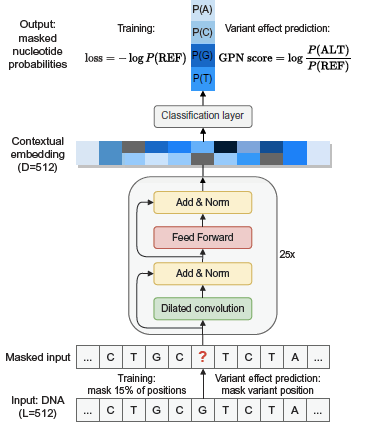
\includegraphics[width=0.5\linewidth,height=\textheight,keepaspectratio]{illustrations/fig_1_kantorovitz.png}

}

\caption{\label{fig-fig_1_kantorovitz}}

\end{figure}%

\chapter{Genome-wide coancestry reveals details of ancient and recent
male-driven reticulation in
baboons}\label{genome-wide-coancestry-reveals-details-of-ancient-and-recent-male-driven-reticulation-in-baboons}

(Knuth 1984)

\begin{Shaded}
\begin{Highlighting}[]
\CommentTok{\# Here is example python code}
\BuiltInTok{print}\NormalTok{(}\StringTok{"Hello world"}\NormalTok{)}
\BuiltInTok{print}\NormalTok{(}\StringTok{"i need to make a update"}\NormalTok{)}
\end{Highlighting}
\end{Shaded}

Here is a reference (Nielsen and Slatkin 2016)

\chapter{References}\label{references}

\phantomsection\label{refs}
\begin{CSLReferences}{1}{0}
\bibitem[\citeproctext]{ref-Kantorovitz2024}
Benegas, Gonzalo, Sanjit Singh Batra, and Yun S. Song. 2024. {``DNA
Language Models Are Powerful Predictors of Genome-Wide Variant
Effects.''} \emph{PNAS}. \url{https://doi.org/10.1073/pnas.2311219121}.

\bibitem[\citeproctext]{ref-knuth84}
Knuth, Donald E. 1984. {``Literate Programming.''} \emph{Comput. J.} 27
(2): 97--111. \url{https://doi.org/10.1093/comjnl/27.2.97}.

\bibitem[\citeproctext]{ref-NielsenSlatkin2016}
Nielsen, Rasmgb, and Montgomery Slatkin. 2016. \emph{An Introduction to
Population Genetics: Theory and Applications}.

\end{CSLReferences}


\backmatter


\end{document}
